\documentclass[11pt]{article}

\usepackage{amsmath,amssymb}
\usepackage[margin=0.9in]{geometry}
\usepackage{booktabs}
\usepackage{caption}
\usepackage{graphicx}
\usepackage[colorlinks=true,linkcolor=blue,citecolor=blue,urlcolor=blue]{hyperref}

\graphicspath{{../experiments/out/supplement/}}

\newcommand{\norm}[1]{\left\lVert #1 \right\rVert}
\newcommand{\ROF}{\mathrm{ROF}}
\newcommand{\dv}{\operatorname{div}}

\title{Transport Geometry Fusion Descent:\\ visual supplement\\
\large twenty cartoon + texture decompositions with scale-band separation}
\author{Joshuah Rainstar\\
\texttt{joshuah.rainstar@gmail.com}}
\date{July 21, 2026}

\begin{document}
\maketitle

\section{Contents and protocol}

This supplement provides visual evidence for the companion paper
\emph{Transport Geometry Fusion Descent: a sub-second implementation of
Meyer's $G$-norm cartoon + texture decomposition}. It contains the full
decomposition of twenty standard test images: the twelve images of Set12
(Cameraman, House, Peppers, Starfish, Monarch, Airplane, Parrot, Lena,
Barbara, Boat, Man, Couple) and the first eight images of BSD68.

Each image $f$ is decomposed twice, by the reference method and by ours,
with identical model parameters $\lambda=0.05$, $\mu=40$.

The reference is Algorithm 3 of Gilles and Osher: the alternation
\[
u \leftarrow \ROF(f-v,\lambda),
\qquad
v \leftarrow (f-u)-\ROF(f-u,\,1/\mu),
\]
with each inner ROF problem solved to relative tolerance $10^{-4}$ and the
outer alternation run to relative tolerance $10^{-4}$ from the cold start
$u_0=v_0=0$. We use an optimized implementation of this reference ---
warm-started inner Bregman states across outer passes, texture-side
penalty $\eta=10/\mu$, and threaded FFTs --- which preserves the
algorithm's nesting discipline and its fixed point while reducing its wall
time (on Barbara, from 361\,s for the plain implementation to 17\,s; the
fixed-point residuals of the two agree to within the measurement floor).
All reference timings in this supplement are those of the optimized
implementation; the speedup column therefore understates the advantage
over the plain implementation by roughly an order of magnitude.

Transport geometry fusion descent (TGFD) executes the same alternation as
one warm Split Bregman sweep per subproblem per pass against persistent
auxiliary states, with a wall budget of $0.9\,\mathrm{s}\times
(\text{pixels}/512^2)$. The TGFD texture layer is then divided into scale
bands along the rungs $\mu=\{40,10,2.5\}$ by independent ROF solves,
\[
s_k=\ROF(v,1/\mu_k),\qquad
B_0=s_1-s_0,\quad B_1=s_2-s_1,\quad B_2=v-s_2,
\]
with the coarsest survivor $s_0$ returned to the cartoon. All computation
is single-core NumPy apart from FFT threading; timings appear in
Table~\ref{tab:runs} and in each figure header.

Each of the twenty figures shows nine panels. Top row: the input $f$; the
reference cartoon and texture from Gilles' Algorithm 3. Middle row: the
difference of the two cartoons amplified twenty-fold; the TGFD cartoon
(including $s_0$) and texture. Bottom row: the three scale bands displayed
on $[-30,30]$ --- the coarse band ($\mu\,40\!\to\!10$), which carries
large-scale oscillation and the contour-adjacent content that a
single-$\mu$ decomposition mixes into its texture layer; the mid band
($\mu\,10\!\to\!2.5$), which carries the principal fabric and surface
textures; and the fine band ($\mu<2.5$), which carries the finest detail
and grain. Texture panels are displayed on $[-40,40]$.

Recurring observations across the twenty images:

\begin{itemize}
\item On every image the TGFD layers agree with the reference layers to
$\norm{\Delta u}/\norm{f}$ of order $10^{-2}$ (Table~\ref{tab:runs}); the
amplified difference panels show the disagreement to be edge-adjacent
ripple, invisible at display contrast.
\item The cartoon layers are piecewise-smooth with preserved contours at
every image size, obtained within the stated sub-second budgets
(0.23\,s at $256^2$, 0.53--0.54\,s at $481\times321$, 0.90--0.92\,s at
$512^2$).
\item Contour-adjacent leakage --- the face line and table edge of
Barbara, the tripod of Cameraman, the hull edges of Boat --- concentrates
in the coarse band on every image where it occurs; the mid band carries
the recognizable textures (Barbara's scarf and tablecloth, the grass of
Cameraman, the plumage of Parrot and the BSD68 birds, the wave field of
Boat).
\item The fine band is near-uniform grain on the classic photographs and
becomes structured only where genuine fine texture exists (Barbara's
weave, starfish papillae), consistent with the ramp law of the companion
paper: bands are graded, and content divides by scale with cross-talk
decaying linearly in scale ratio.
\end{itemize}

\begin{table}[h]
\centering
\caption{The twenty runs. Reference = Gilles Algorithm 3, nested inner
solves to tolerance $10^{-4}$, optimized implementation (warm inner
states, $\eta=10/\mu$, threaded FFT). Agreement =
$\norm{u_{\mathrm{TGFD}}-u_{\mathrm{Gilles}}}/\norm{f}$. Ladder = wall
time of the three independent band solves.}
\label{tab:runs}
\begin{tabular}{lrrrrrr}
\toprule
image & size & reference (s) & TGFD (s) & speedup & ladder (s) & agreement\\
\midrule
Cameraman & $256\times256$ & 2.4 & 0.23 & 11$\times$ & 1.2 & $11.5\times10^{-3}$ \\
House & $256\times256$ & 5.4 & 0.23 & 24$\times$ & 1.2 & $13.0\times10^{-3}$ \\
Peppers & $256\times256$ & 3.1 & 0.23 & 14$\times$ & 1.7 & $9.8\times10^{-3}$ \\
Starfish & $256\times256$ & 2.1 & 0.23 & 9$\times$ & 1.3 & $6.0\times10^{-3}$ \\
Monarch & $256\times256$ & 2.4 & 0.23 & 10$\times$ & 1.6 & $6.1\times10^{-3}$ \\
Airplane & $256\times256$ & 2.7 & 0.23 & 12$\times$ & 1.1 & $4.9\times10^{-3}$ \\
Parrot & $256\times256$ & 2.5 & 0.23 & 11$\times$ & 1.2 & $6.4\times10^{-3}$ \\
Lena & $512\times512$ & 16.9 & 0.92 & 18$\times$ & 6.6 & $13.1\times10^{-3}$ \\
Barbara & $512\times512$ & 14.5 & 0.90 & 16$\times$ & 6.1 & $7.7\times10^{-3}$ \\
Boat & $512\times512$ & 11.4 & 0.90 & 13$\times$ & 5.3 & $7.2\times10^{-3}$ \\
Man & $512\times512$ & 13.1 & 0.91 & 14$\times$ & 7.0 & $7.9\times10^{-3}$ \\
Couple & $512\times512$ & 11.8 & 0.90 & 13$\times$ & 5.6 & $8.4\times10^{-3}$ \\
BSD68-01 & $481\times321$ & 7.8 & 0.53 & 15$\times$ & 4.3 & $12.9\times10^{-3}$ \\
BSD68-02 & $481\times321$ & 14.4 & 0.54 & 27$\times$ & 4.4 & $13.9\times10^{-3}$ \\
BSD68-03 & $481\times321$ & 7.9 & 0.53 & 15$\times$ & 4.4 & $12.8\times10^{-3}$ \\
BSD68-04 & $321\times481$ & 8.2 & 0.53 & 15$\times$ & 3.8 & $7.5\times10^{-3}$ \\
BSD68-05 & $321\times481$ & 8.6 & 0.54 & 16$\times$ & 3.9 & $7.4\times10^{-3}$ \\
BSD68-06 & $321\times481$ & 10.9 & 0.54 & 20$\times$ & 3.9 & $14.3\times10^{-3}$ \\
BSD68-07 & $321\times481$ & 6.4 & 0.53 & 12$\times$ & 3.7 & $8.3\times10^{-3}$ \\
BSD68-08 & $321\times481$ & 7.1 & 0.54 & 13$\times$ & 4.4 & $7.8\times10^{-3}$ \\
\bottomrule
\end{tabular}
\end{table}

\clearpage
\section{Set12}

\begin{center}
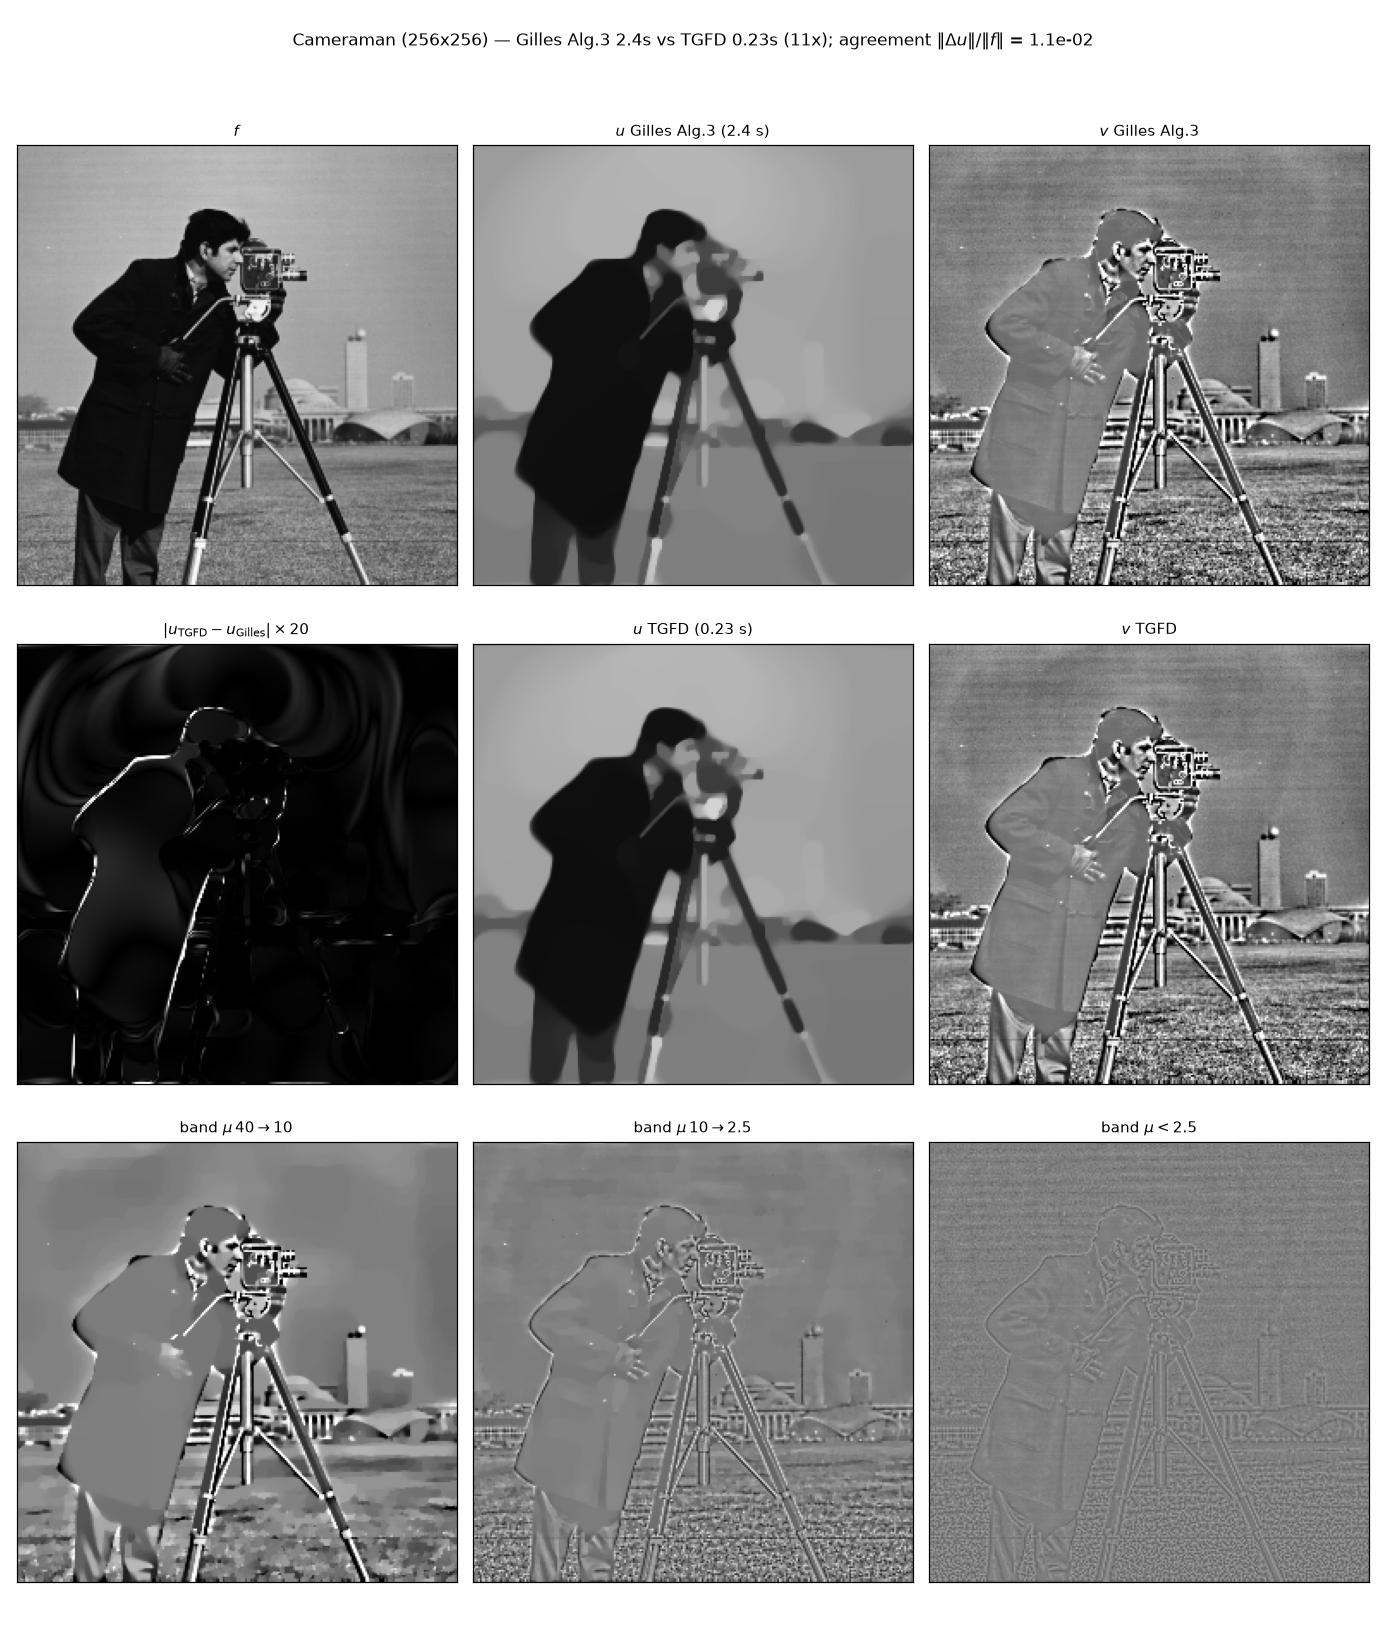
\includegraphics[width=\textwidth,height=0.9\textheight,keepaspectratio]{set12_01.png}
\captionof{figure}{Cameraman, $256^2$. The grass field divides between the mid and
fine bands; the tripod's contour leakage sits in the coarse band.}
\end{center}
\clearpage

\begin{center}
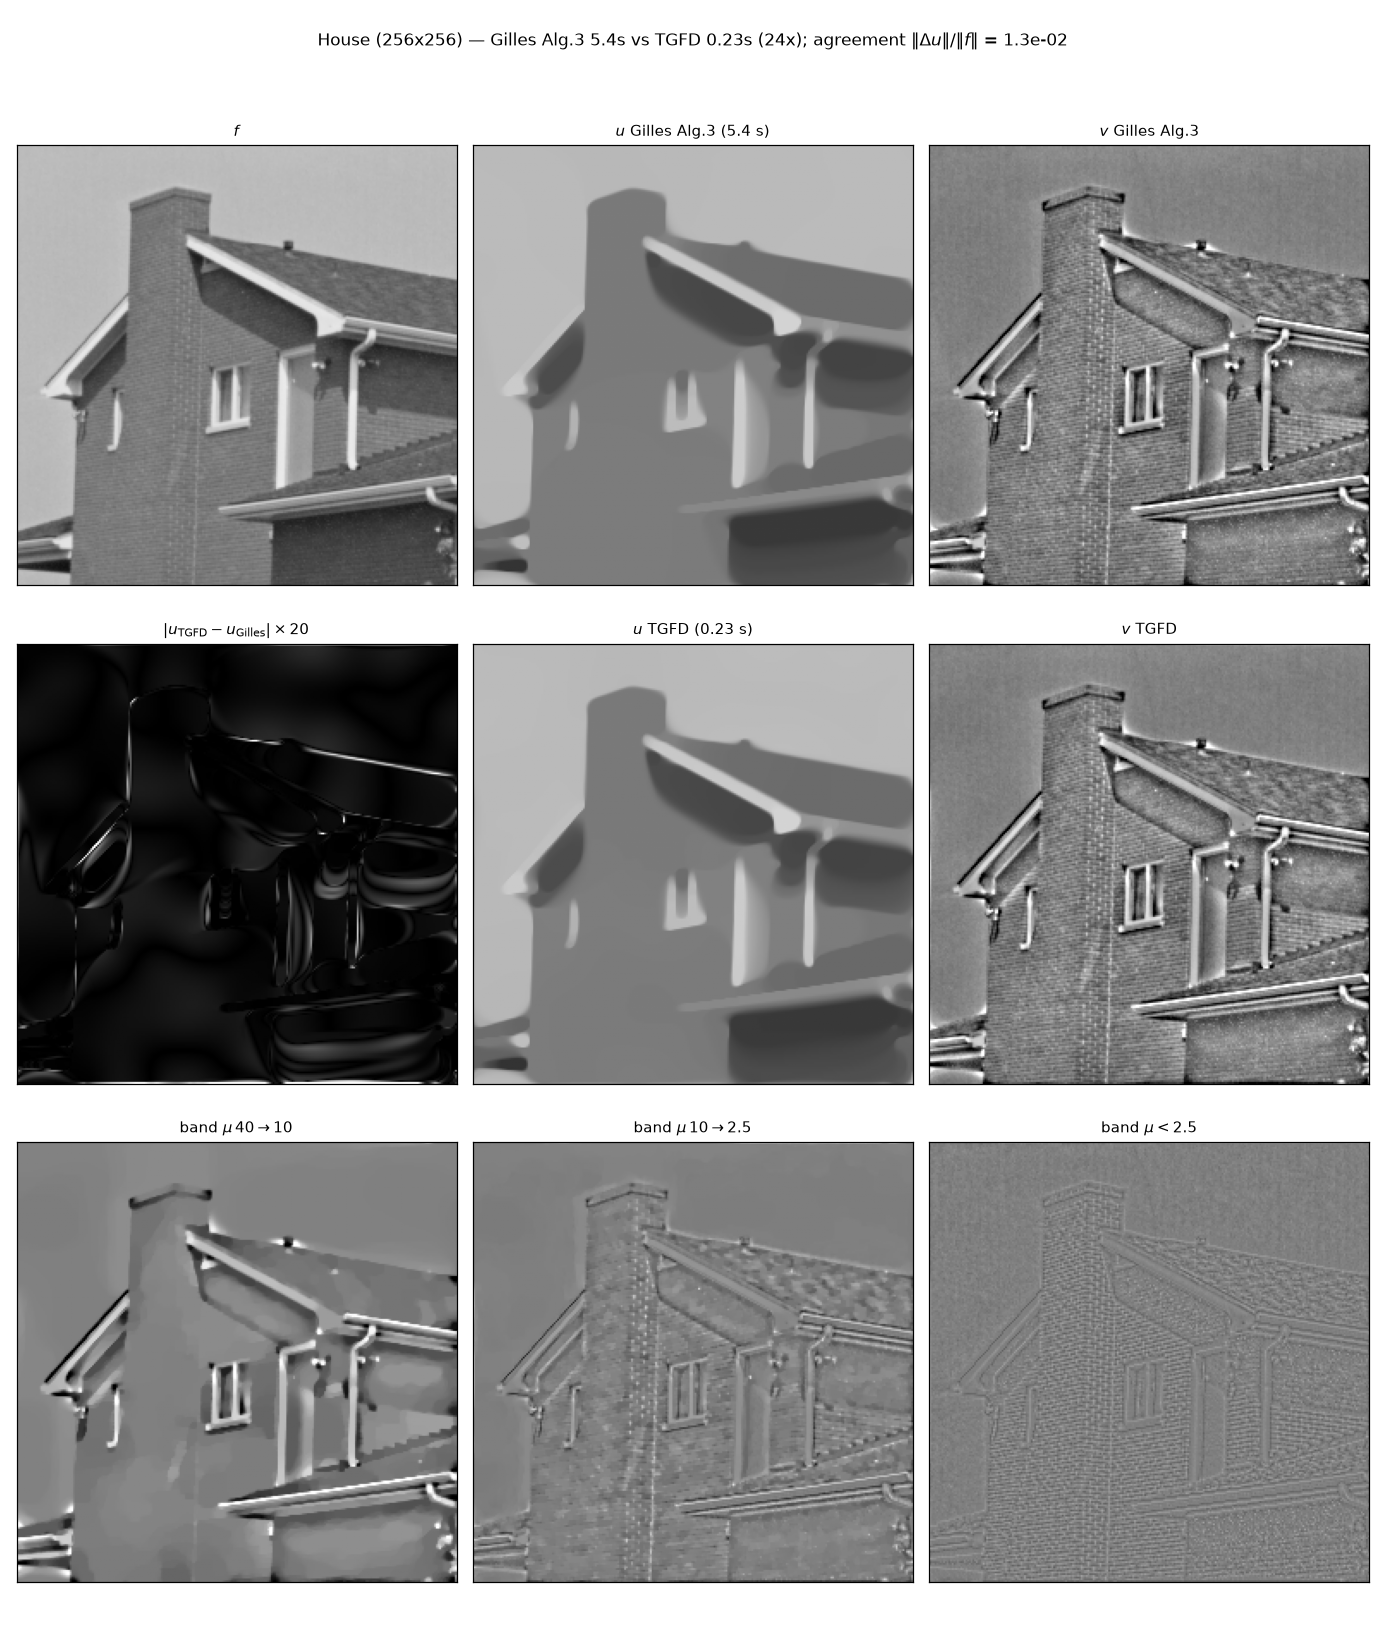
\includegraphics[width=\textwidth,height=0.9\textheight,keepaspectratio]{set12_02.png}
\captionof{figure}{House, $256^2$. The brickwork and shingles appear in the mid
band; the roof line and gutter contours in the coarse band.}
\end{center}
\clearpage

\begin{center}
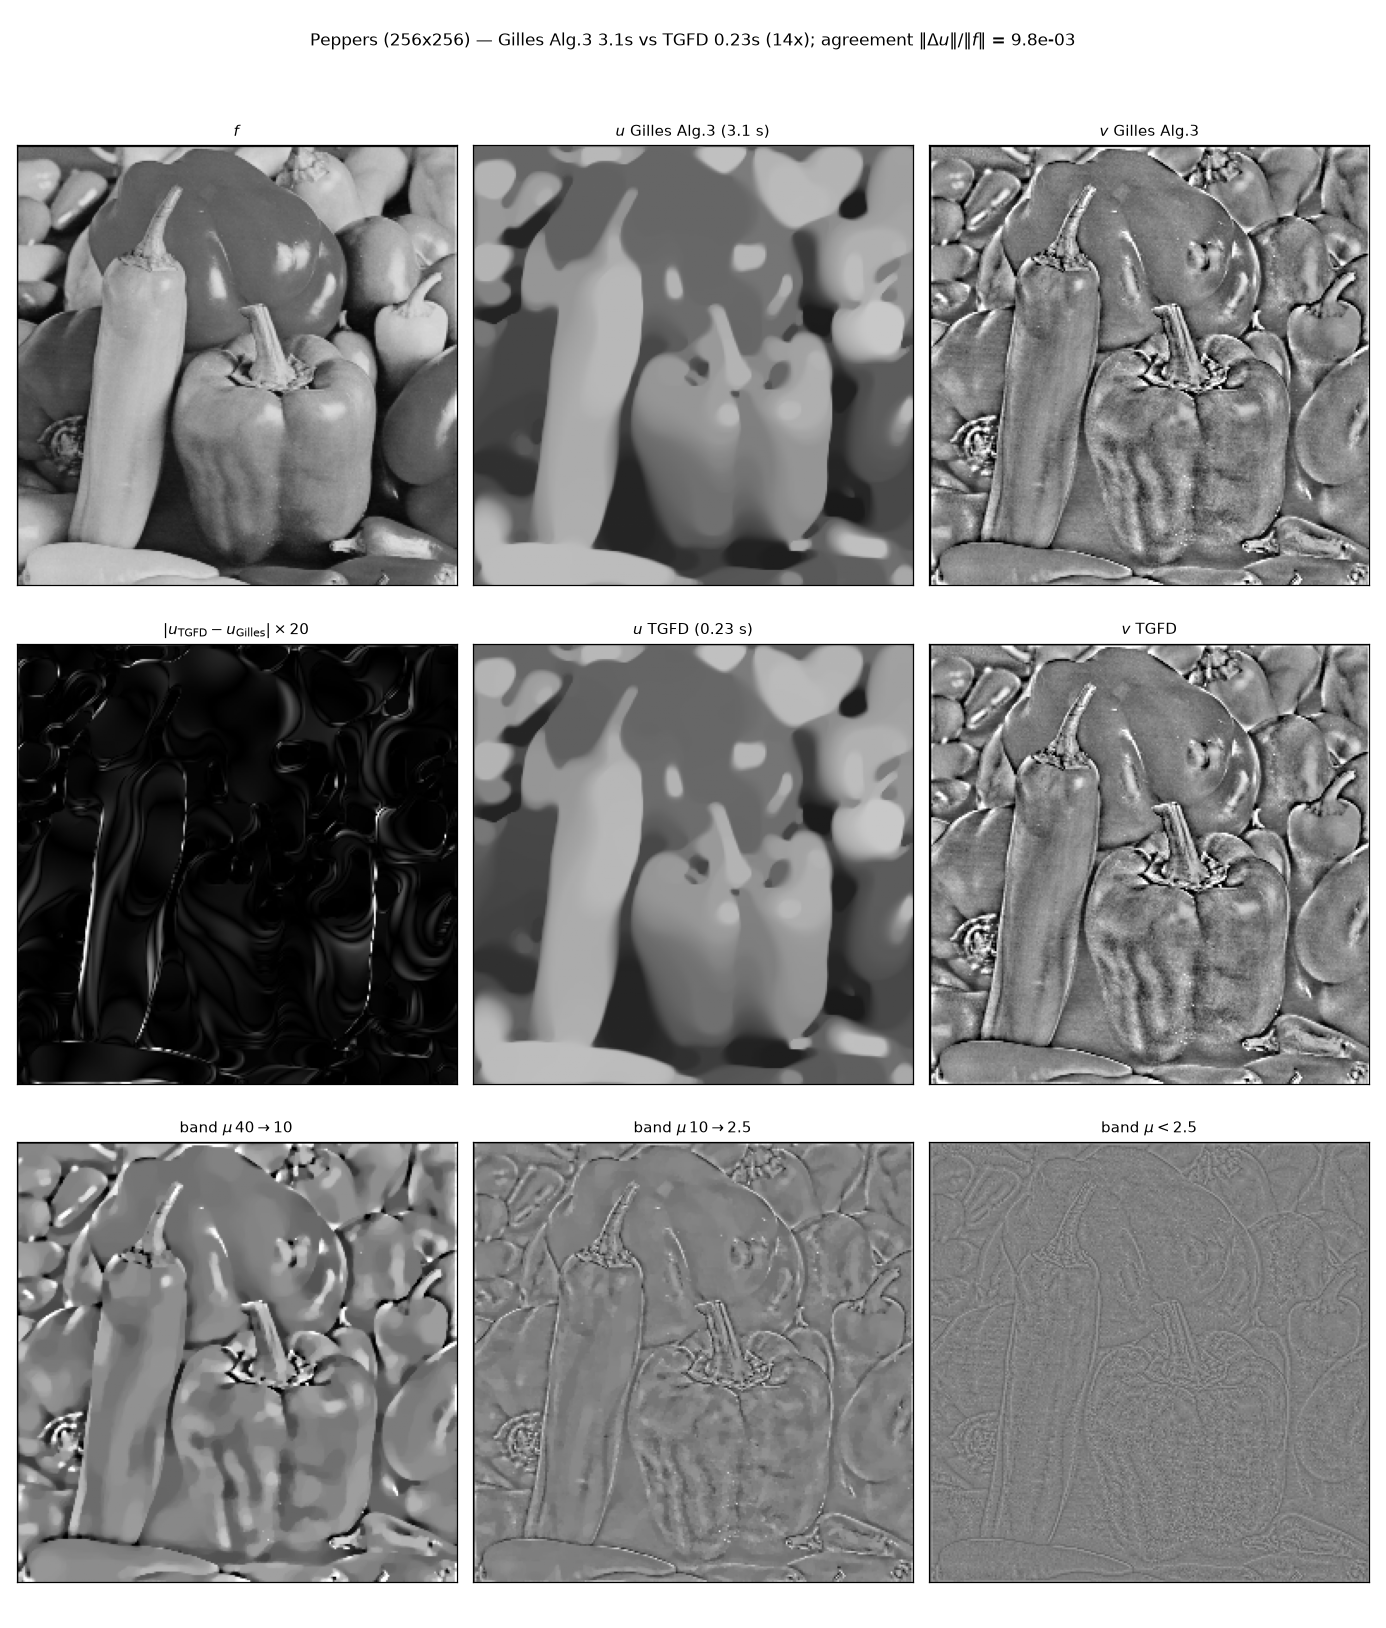
\includegraphics[width=\textwidth,height=0.9\textheight,keepaspectratio]{set12_03.png}
\captionof{figure}{Peppers, $256^2$. A near-cartoon image: the texture layer is
thin, and the bands contain principally specular detail and grain.}
\end{center}
\clearpage

\begin{center}
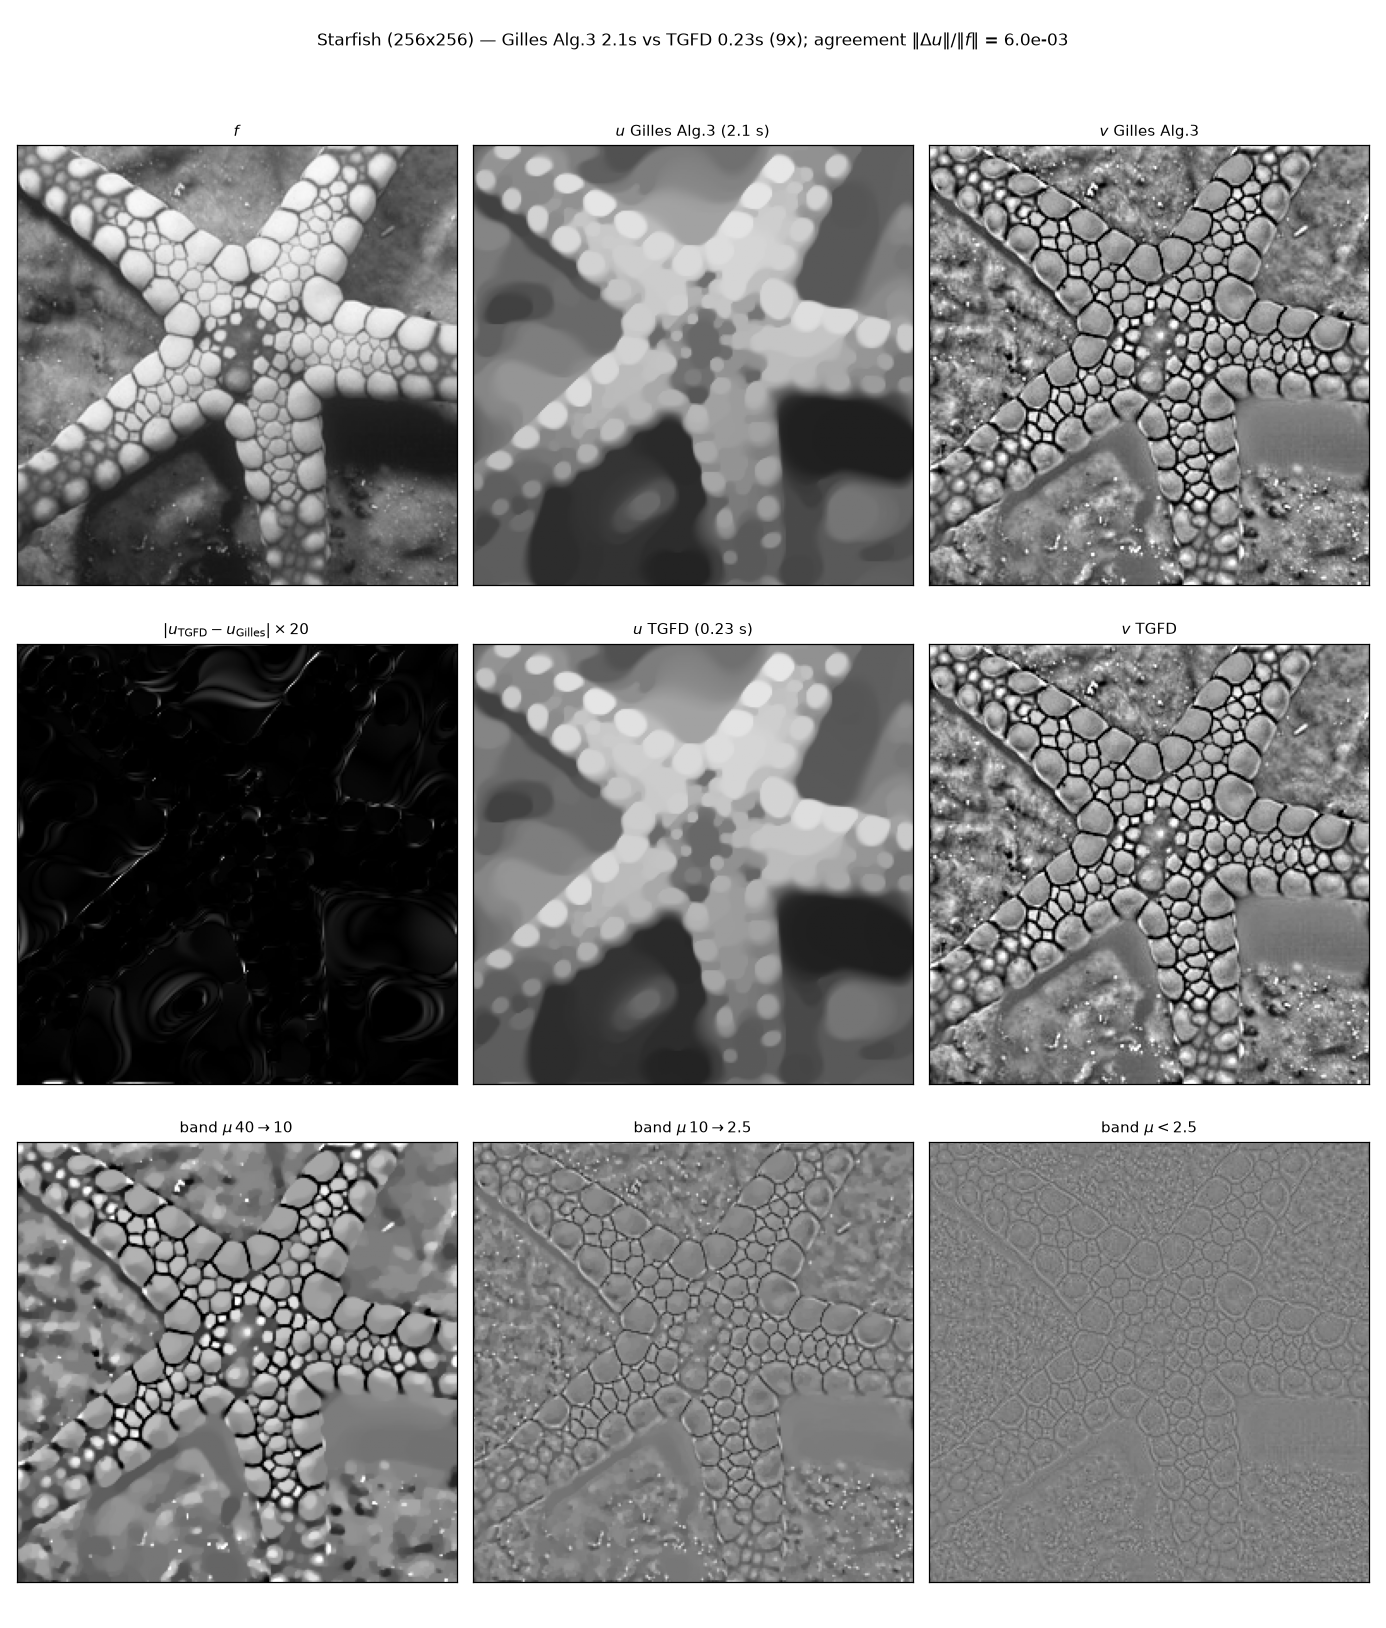
\includegraphics[width=\textwidth,height=0.9\textheight,keepaspectratio]{set12_04.png}
\captionof{figure}{Starfish, $256^2$. The papillae pattern is genuine fine-scale
texture and populates the mid and fine bands; the arm outlines remain in
the coarse band.}
\end{center}
\clearpage

\begin{center}
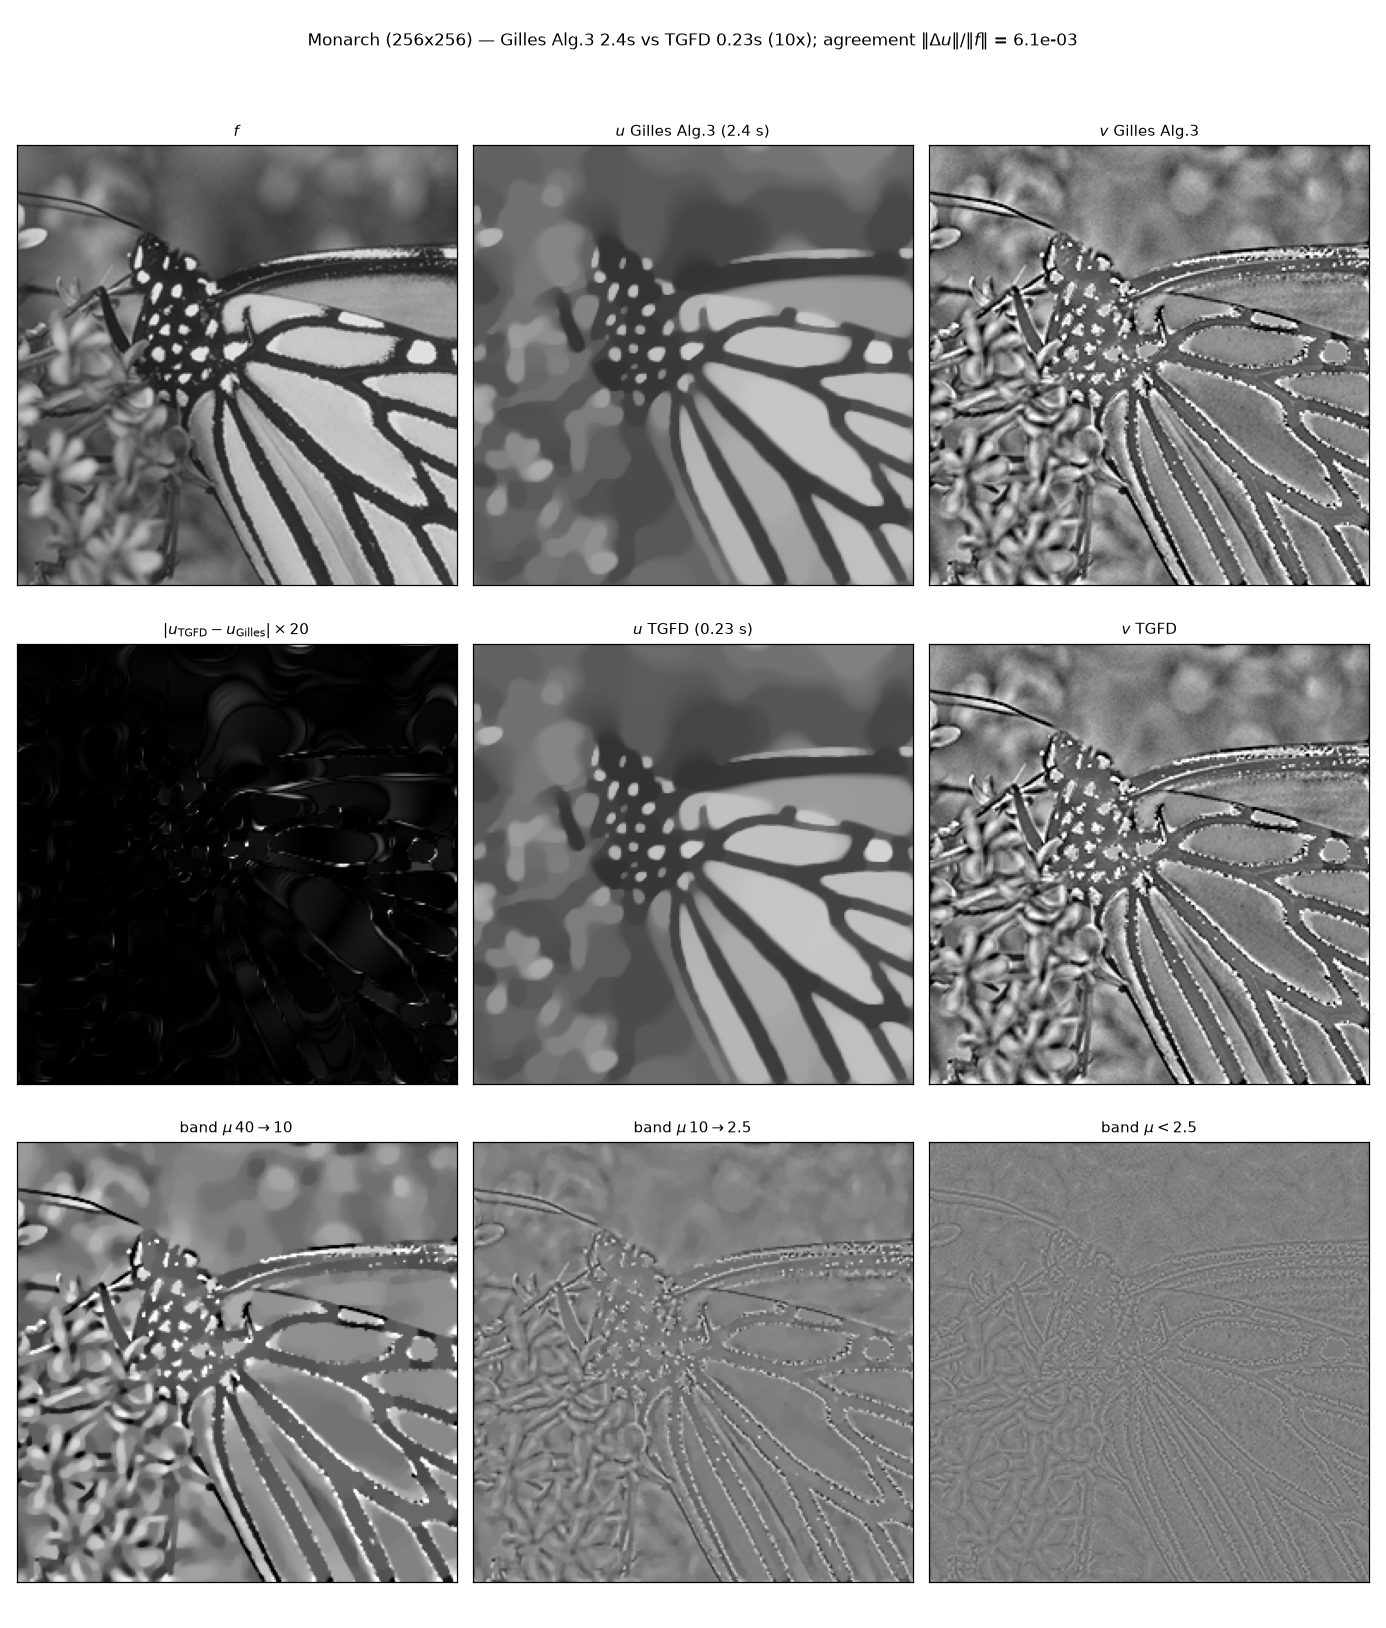
\includegraphics[width=\textwidth,height=0.9\textheight,keepaspectratio]{set12_05.png}
\captionof{figure}{Monarch, $256^2$. Wing venation in the coarse and mid bands;
the flower texture divides by scale.}
\end{center}
\clearpage

\begin{center}
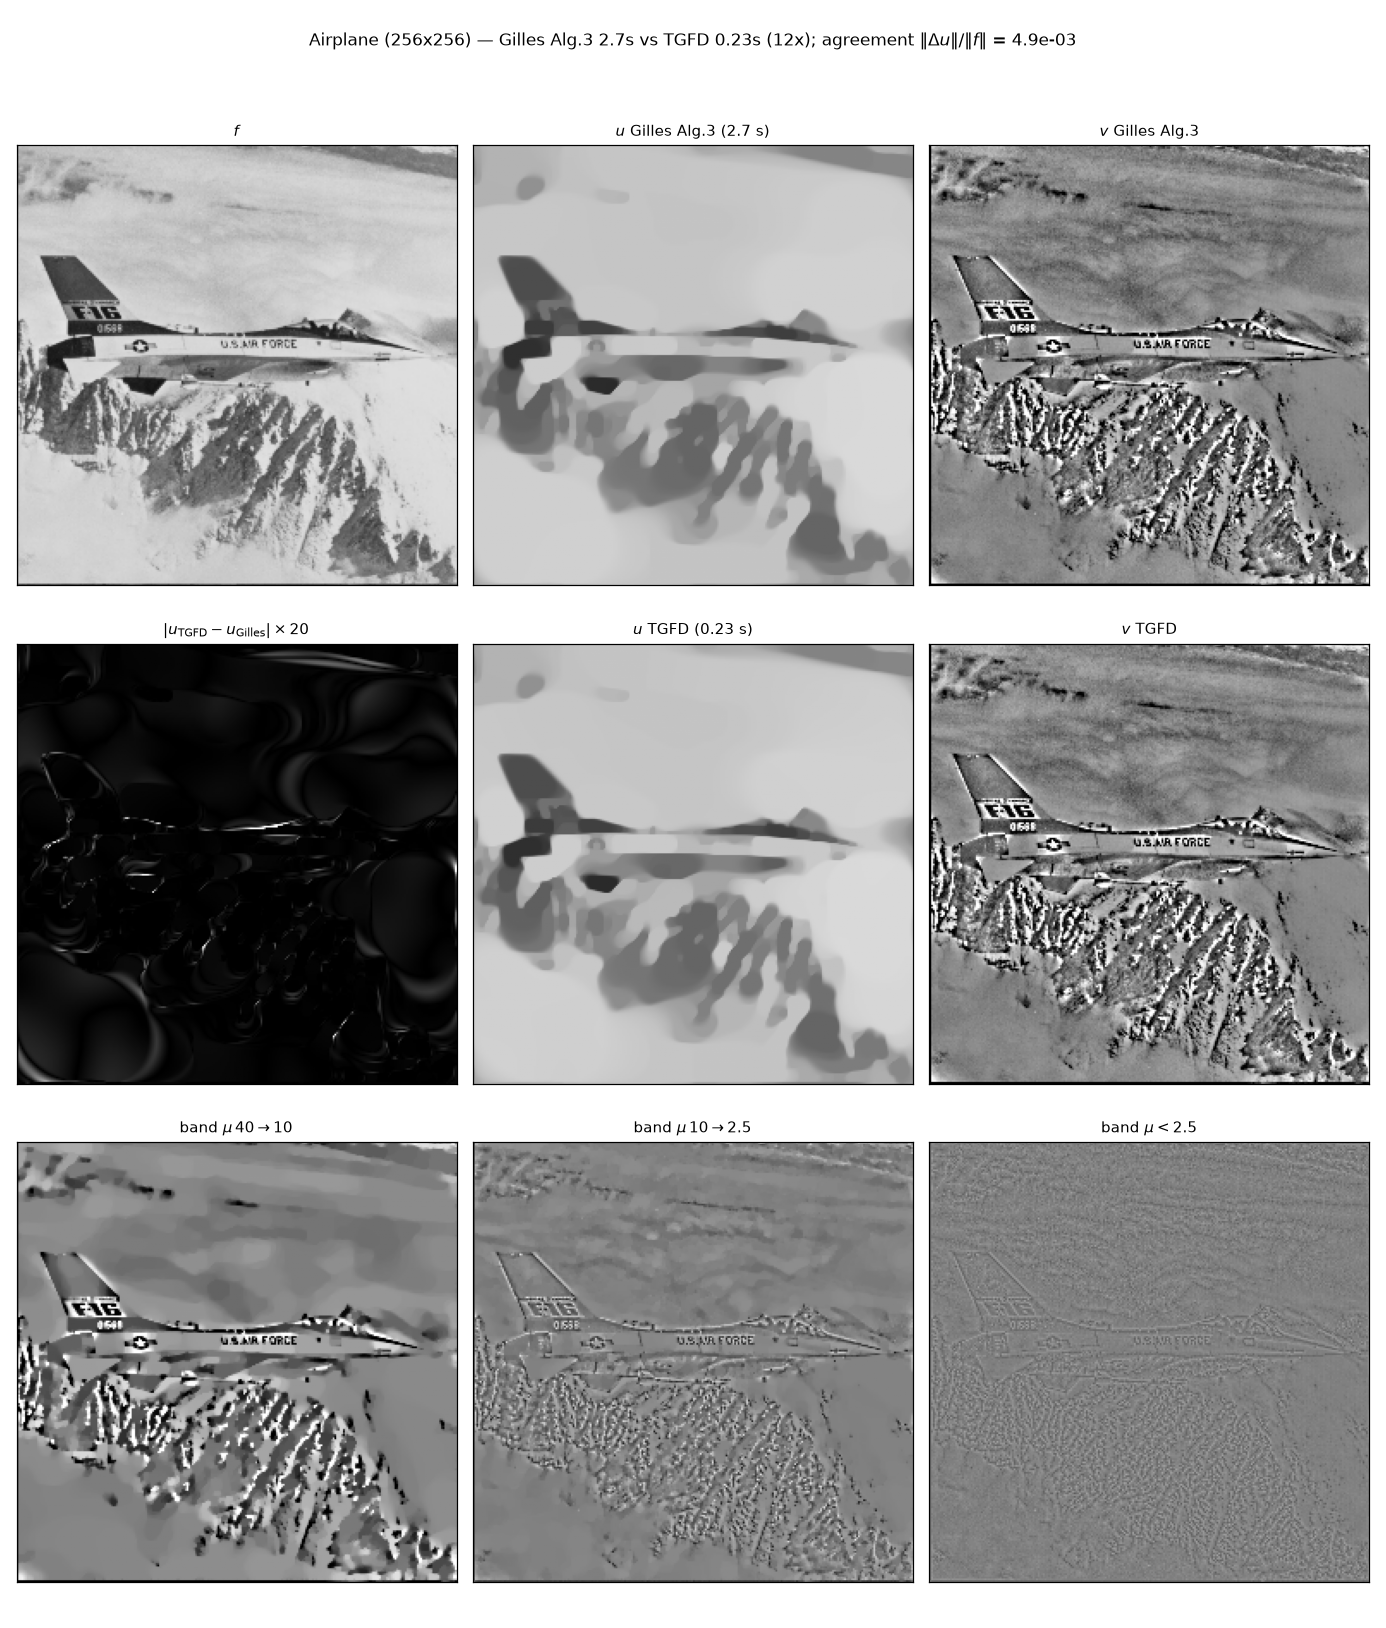
\includegraphics[width=\textwidth,height=0.9\textheight,keepaspectratio]{set12_06.png}
\captionof{figure}{Airplane, $256^2$. Lettering and insignia --- oscillatory at the
scale of the $\mu$-ball --- enter the texture layer and sort into the
coarse and mid bands.}
\end{center}
\clearpage

\begin{center}
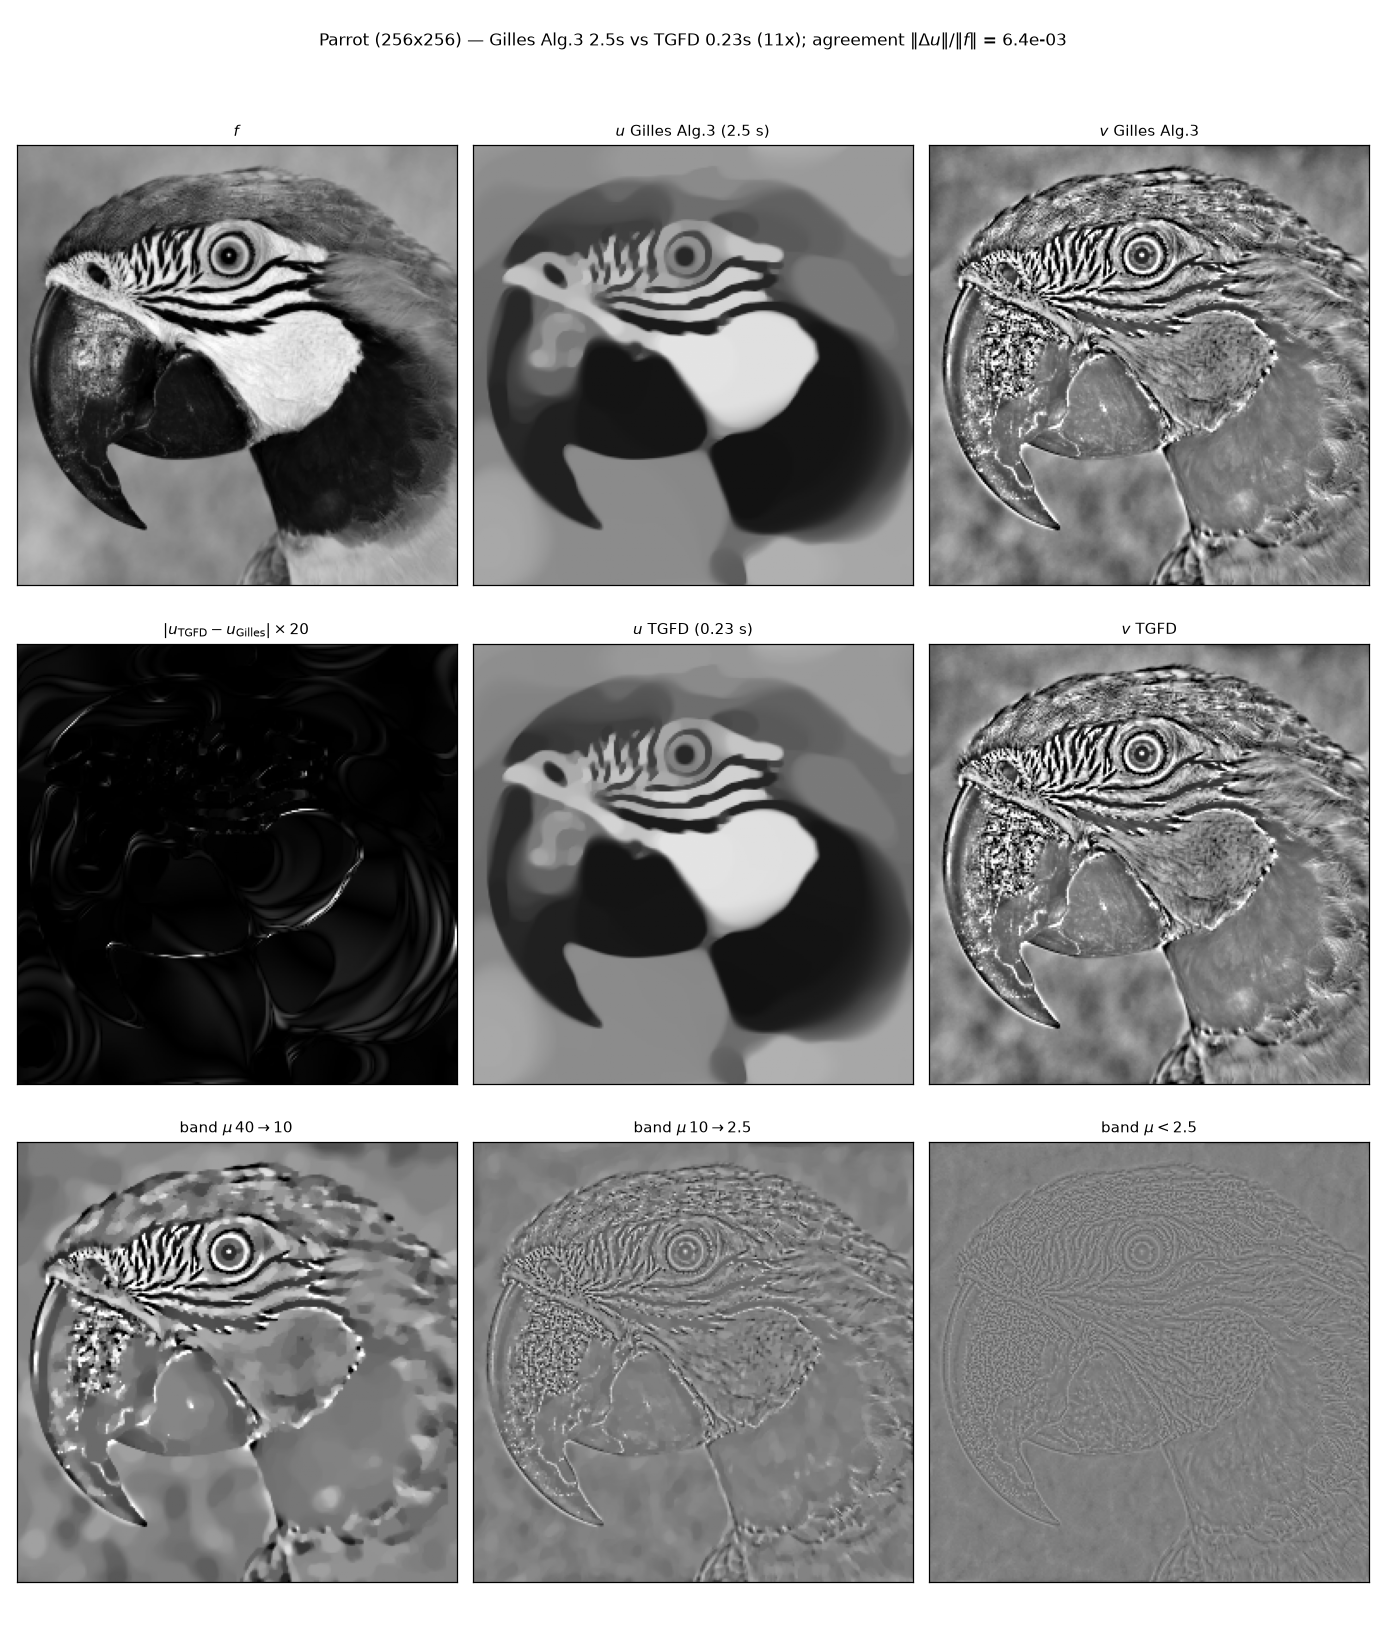
\includegraphics[width=\textwidth,height=0.9\textheight,keepaspectratio]{set12_07.png}
\captionof{figure}{Parrot, $256^2$. Facial barring in the mid band; the beak and
eye contours in the coarse band; feather grain in the fine band.}
\end{center}
\clearpage

\begin{center}
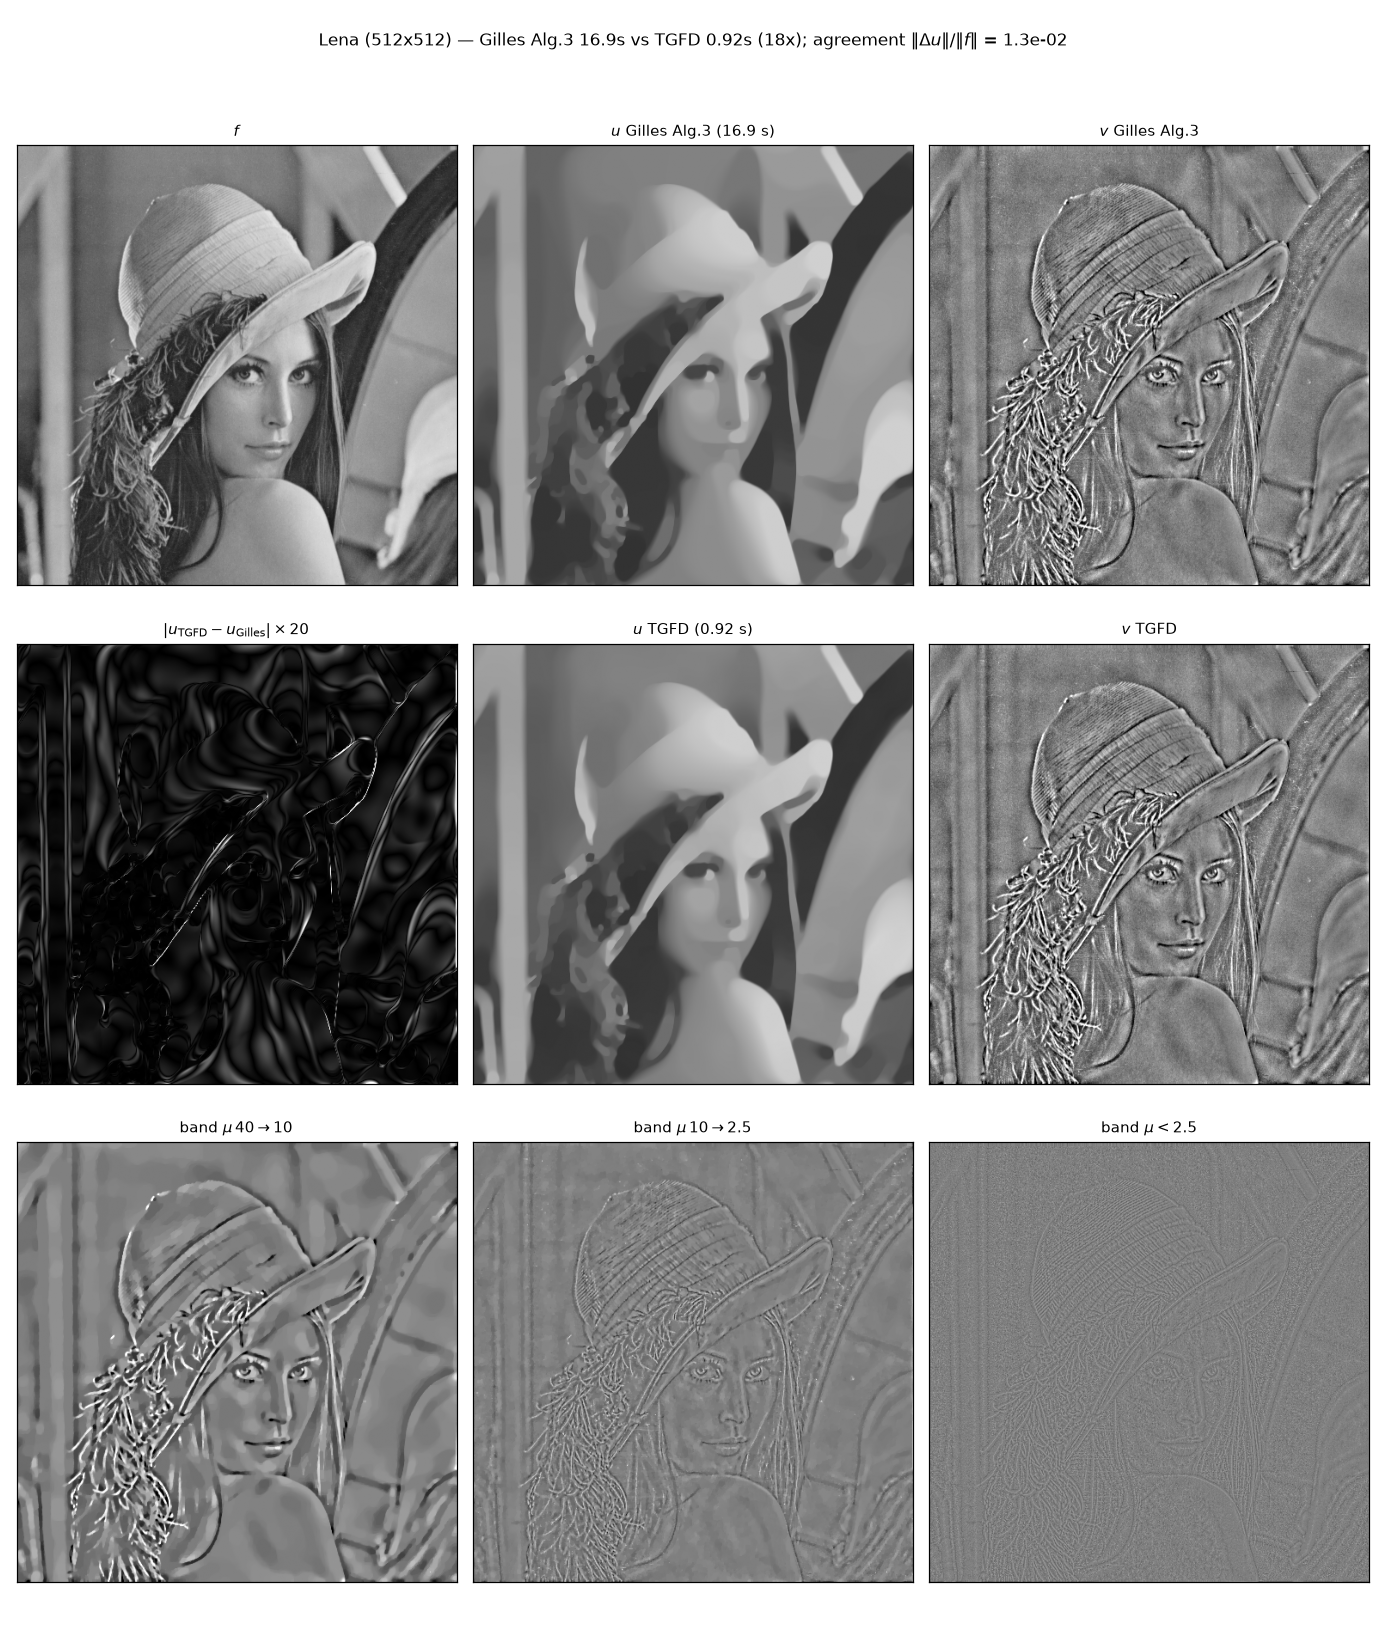
\includegraphics[width=\textwidth,height=0.9\textheight,keepaspectratio]{set12_08.png}
\captionof{figure}{Lena, $512^2$. The hat's straw texture and feather boa populate
the coarse and mid bands; skin regions contribute almost nothing to the
texture layer, as the model intends.}
\end{center}
\clearpage

\begin{center}
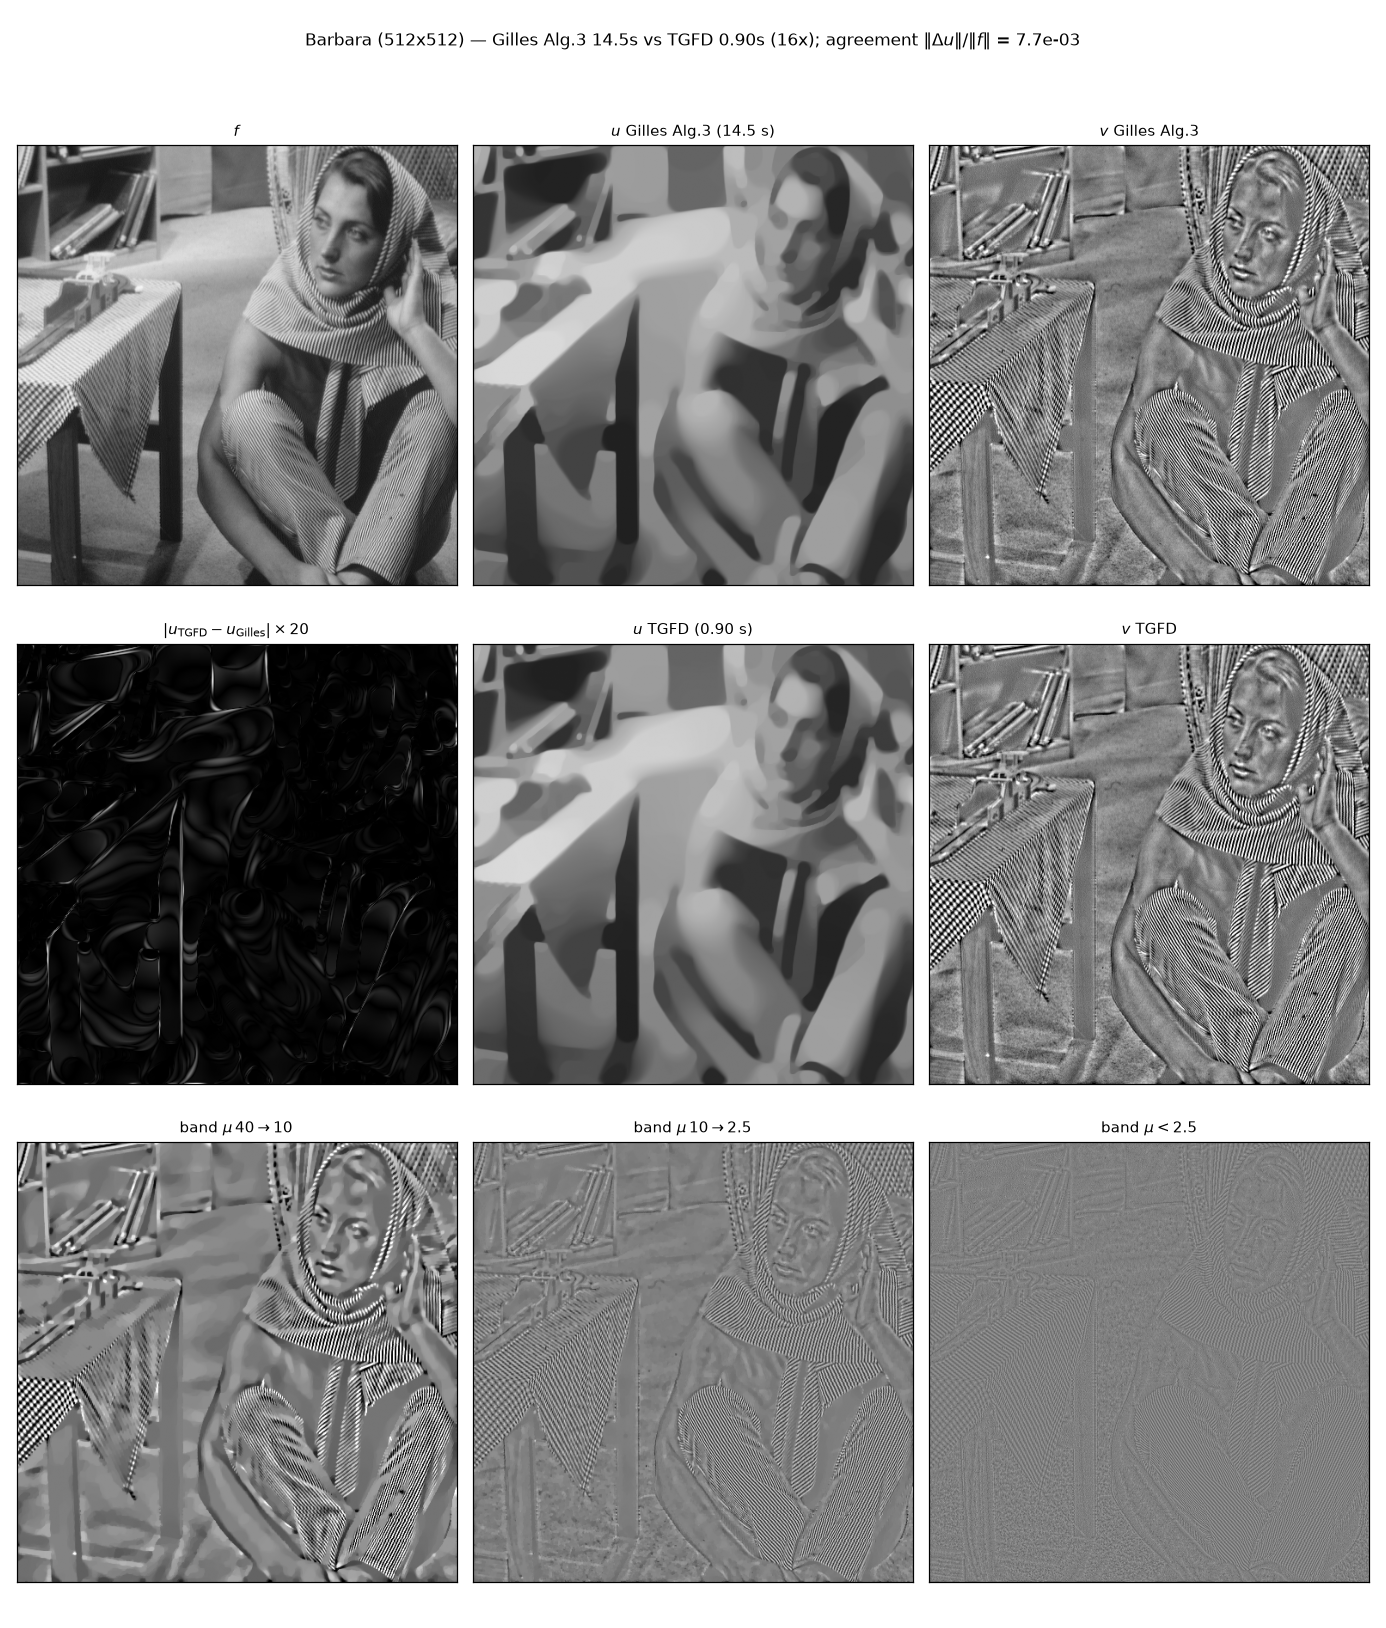
\includegraphics[width=\textwidth,height=0.9\textheight,keepaspectratio]{set12_09.png}
\captionof{figure}{Barbara, $512^2$. The image of the companion paper: scarf
stripes and tablecloth check in the mid band; face-line and table-edge
leakage confined to the coarse band; weave and grain in the fine band.}
\end{center}
\clearpage

\begin{center}
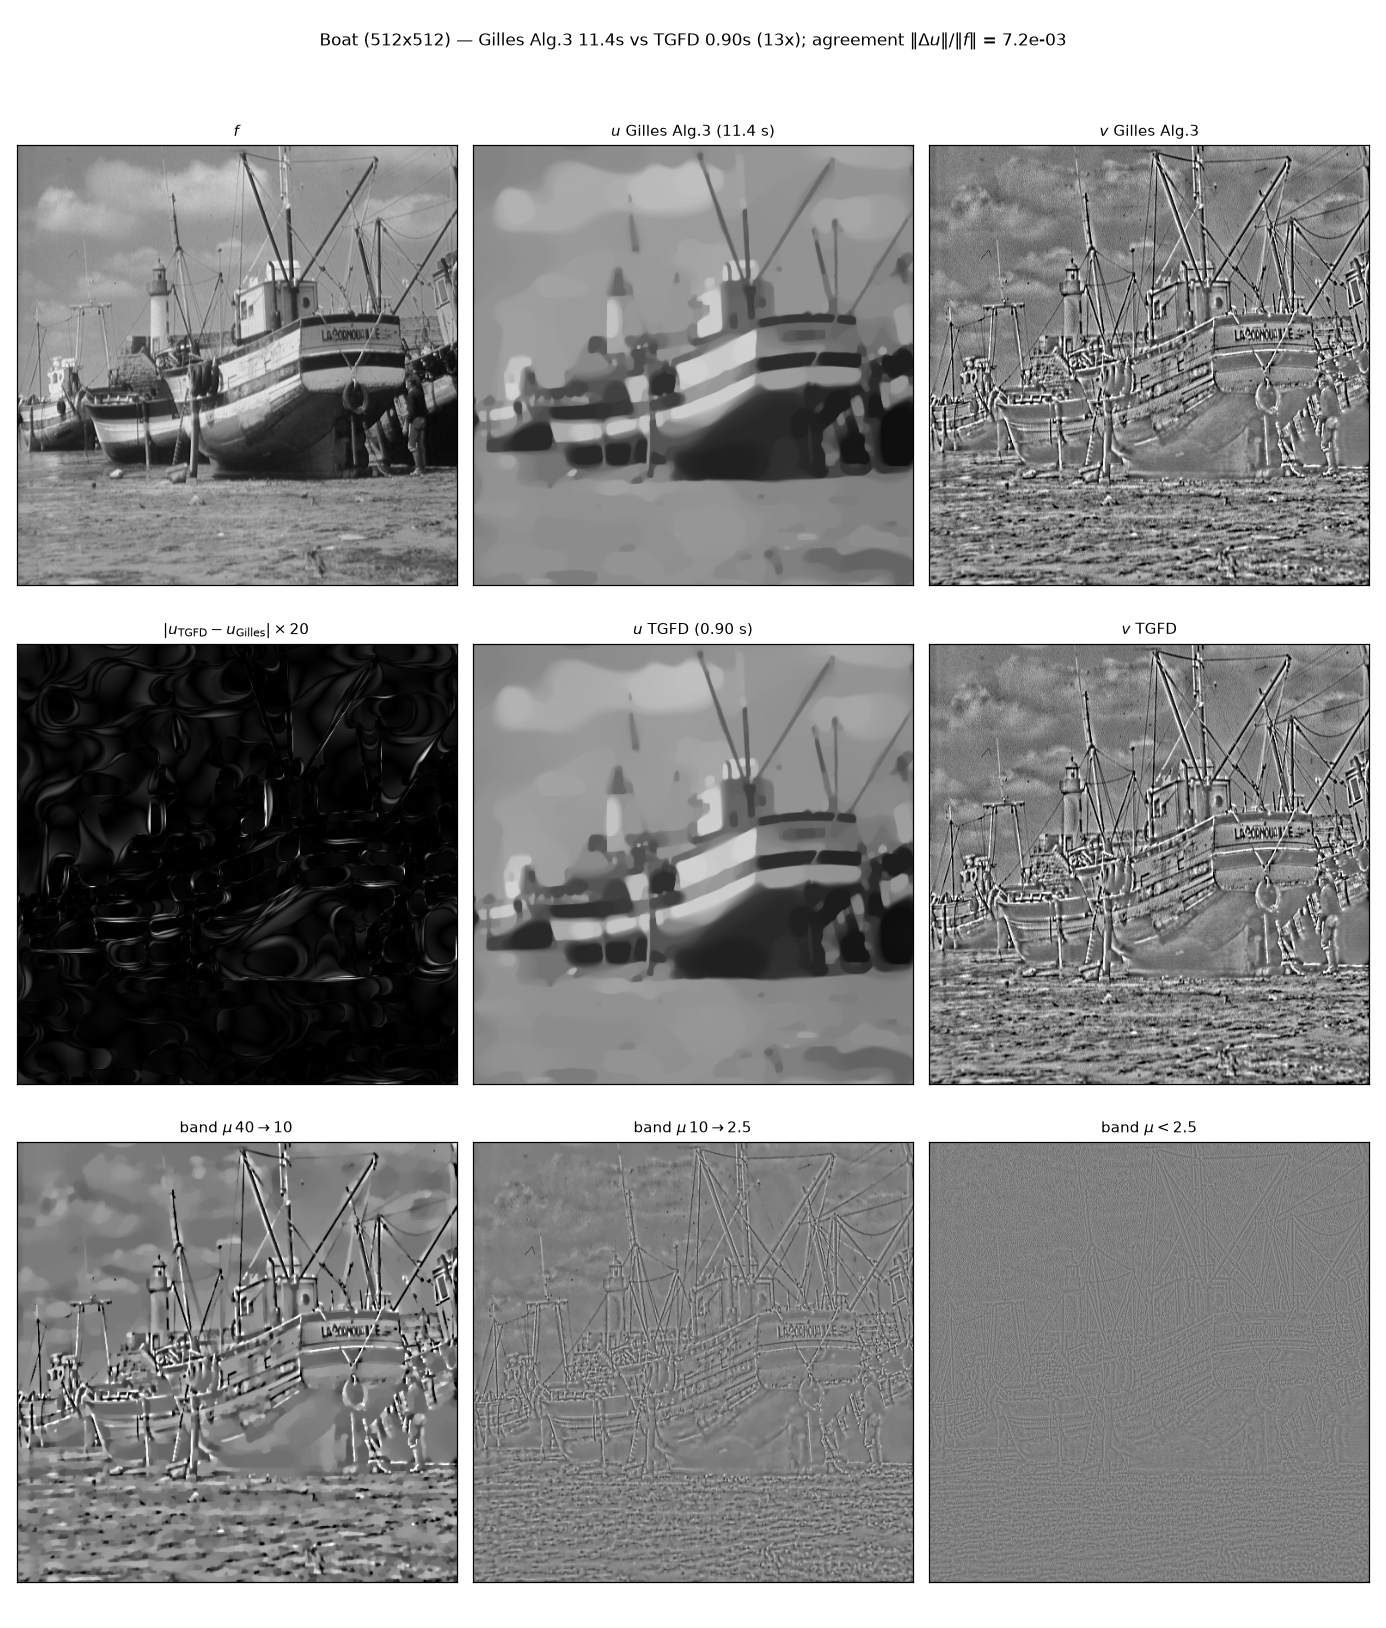
\includegraphics[width=\textwidth,height=0.9\textheight,keepaspectratio]{set12_10.png}
\captionof{figure}{Boat, $512^2$. The wave field and deck planking in the mid band;
mast and hull contour leakage in the coarse band.}
\end{center}
\clearpage

\begin{center}
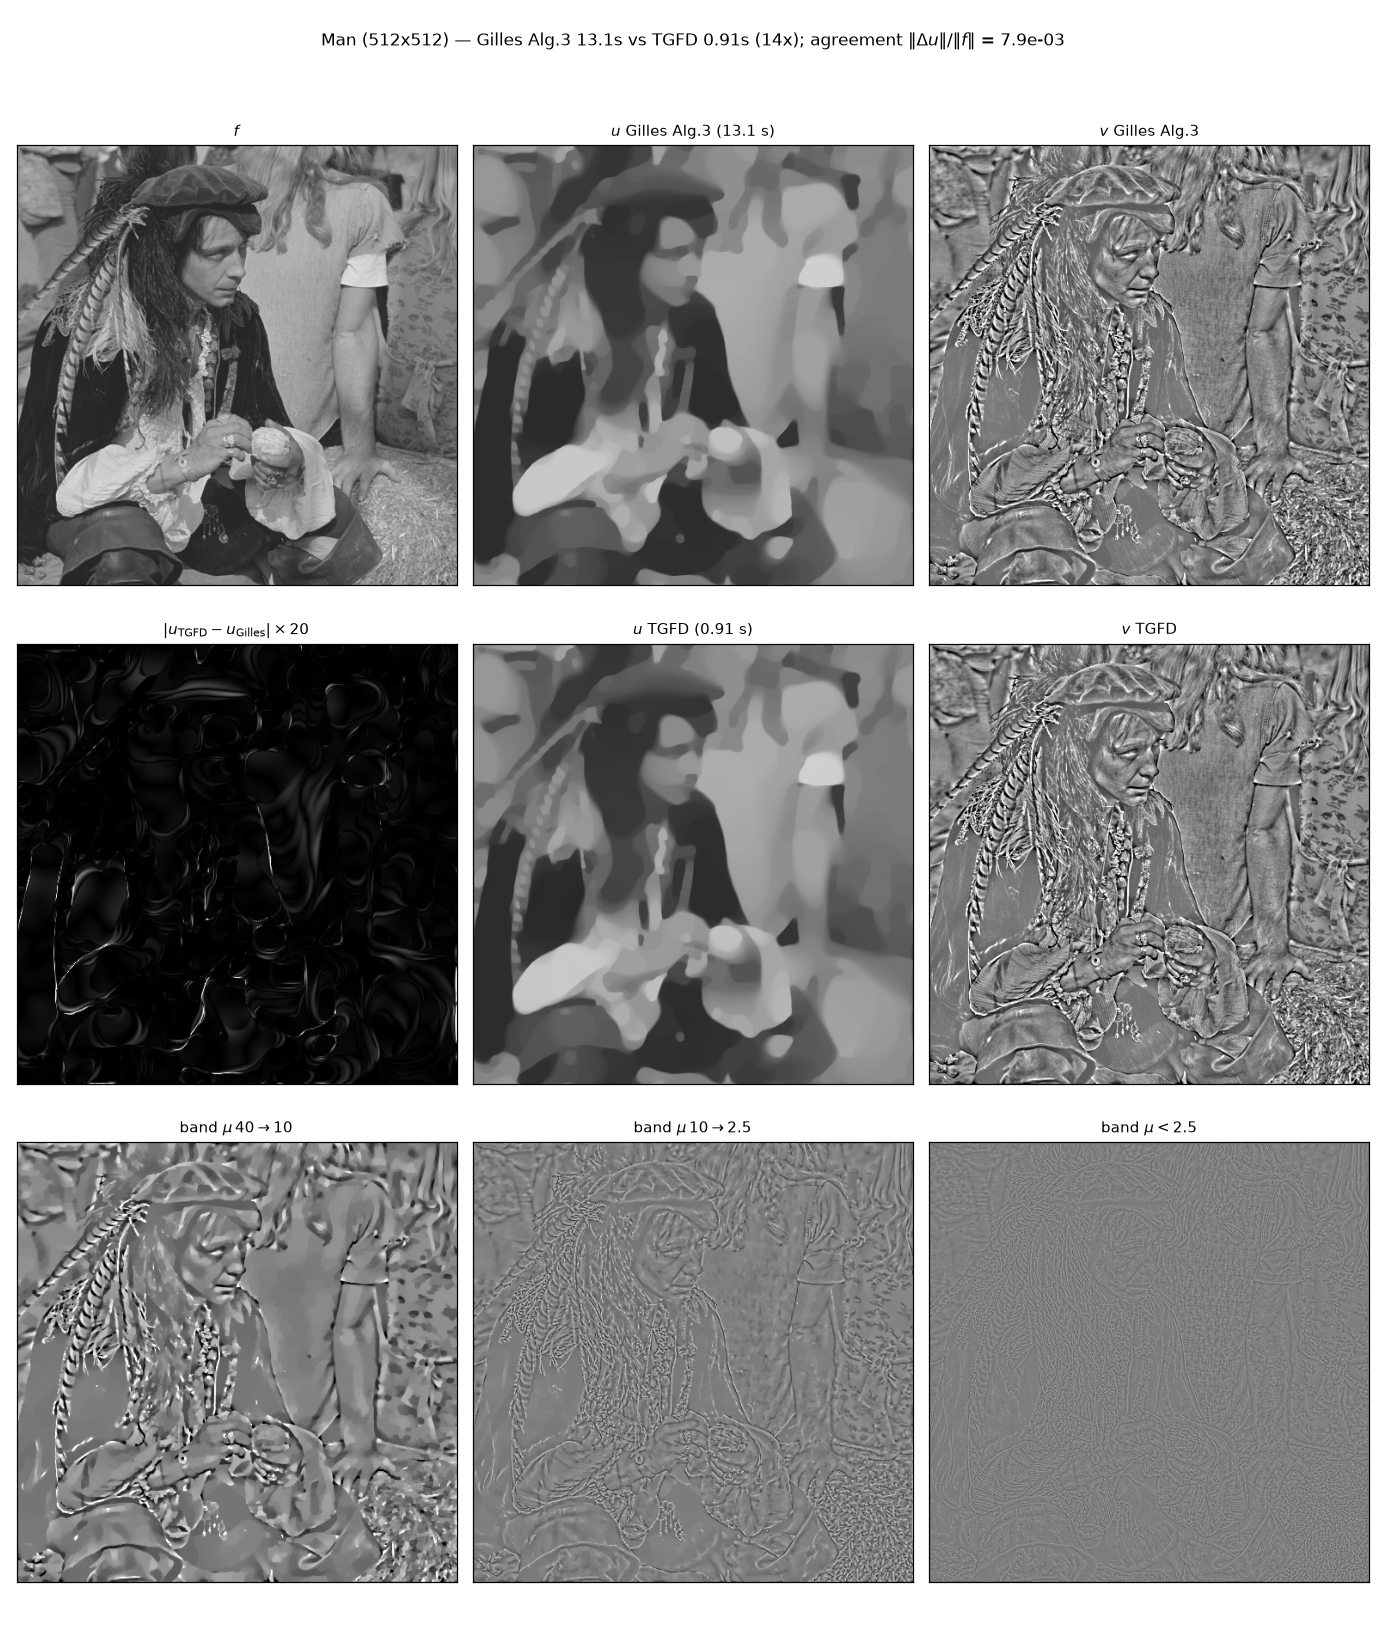
\includegraphics[width=\textwidth,height=0.9\textheight,keepaspectratio]{set12_11.png}
\captionof{figure}{Man, $512^2$. Hair and fabric in the mid band; the fine band is
principally film grain, uniform across the frame.}
\end{center}
\clearpage

\begin{center}
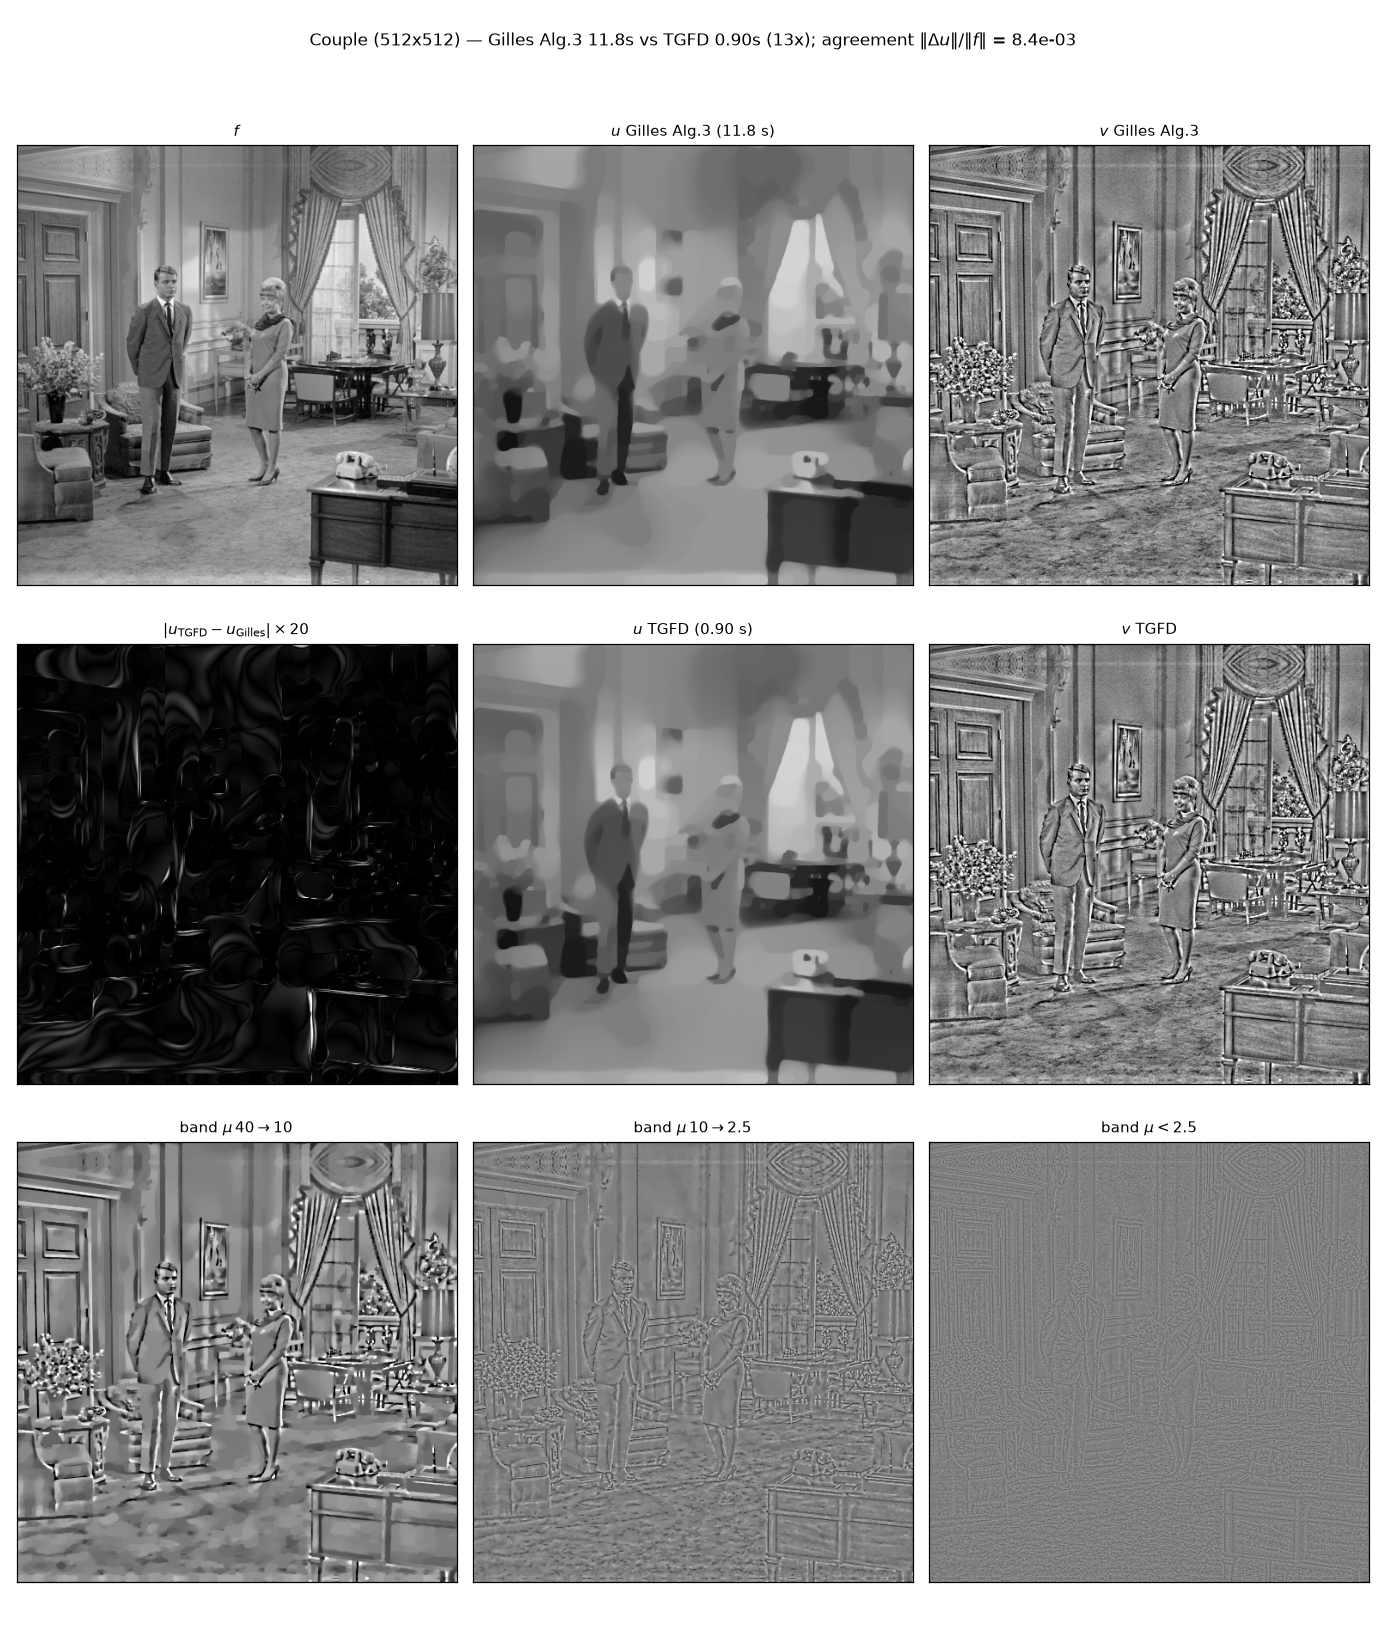
\includegraphics[width=\textwidth,height=0.9\textheight,keepaspectratio]{set12_12.png}
\captionof{figure}{Couple, $512^2$. Clothing textures in the mid band; furniture
contours in the coarse band.}
\end{center}
\clearpage

\clearpage
\section{BSD68 (first eight)}

\begin{center}
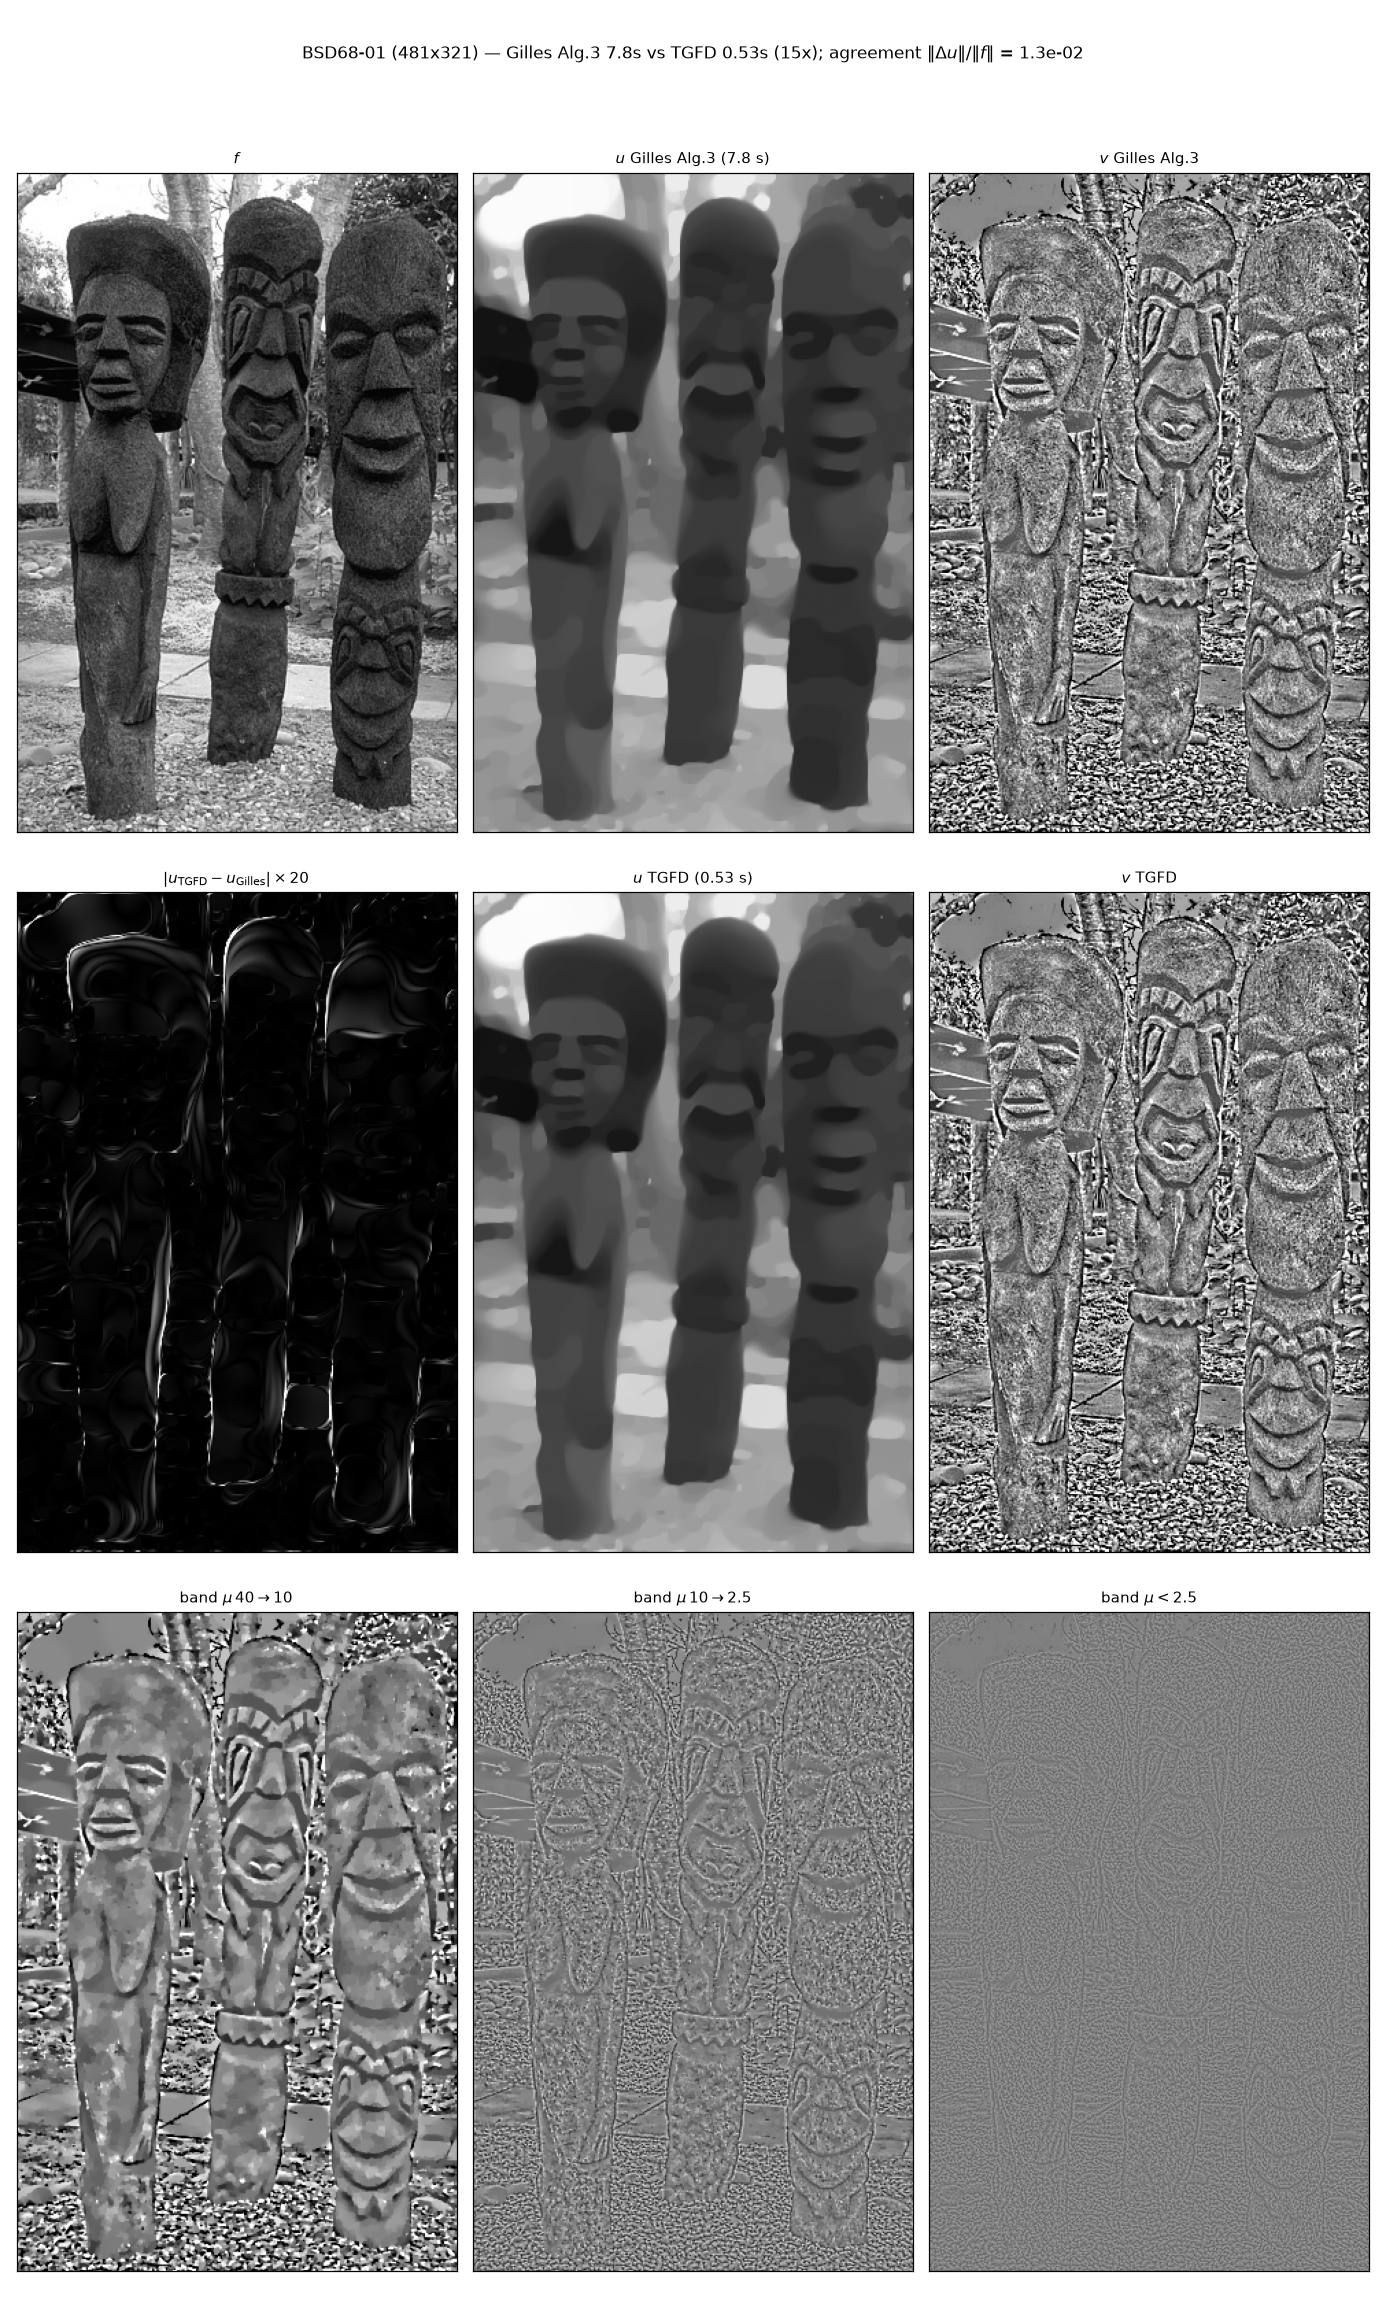
\includegraphics[width=\textwidth,height=0.9\textheight,keepaspectratio]{bsd68_001.png}
\captionof{figure}{BSD68-01, $481\times321$. Natural foliage texture divides
between the mid and fine bands.}
\end{center}
\clearpage

\begin{center}
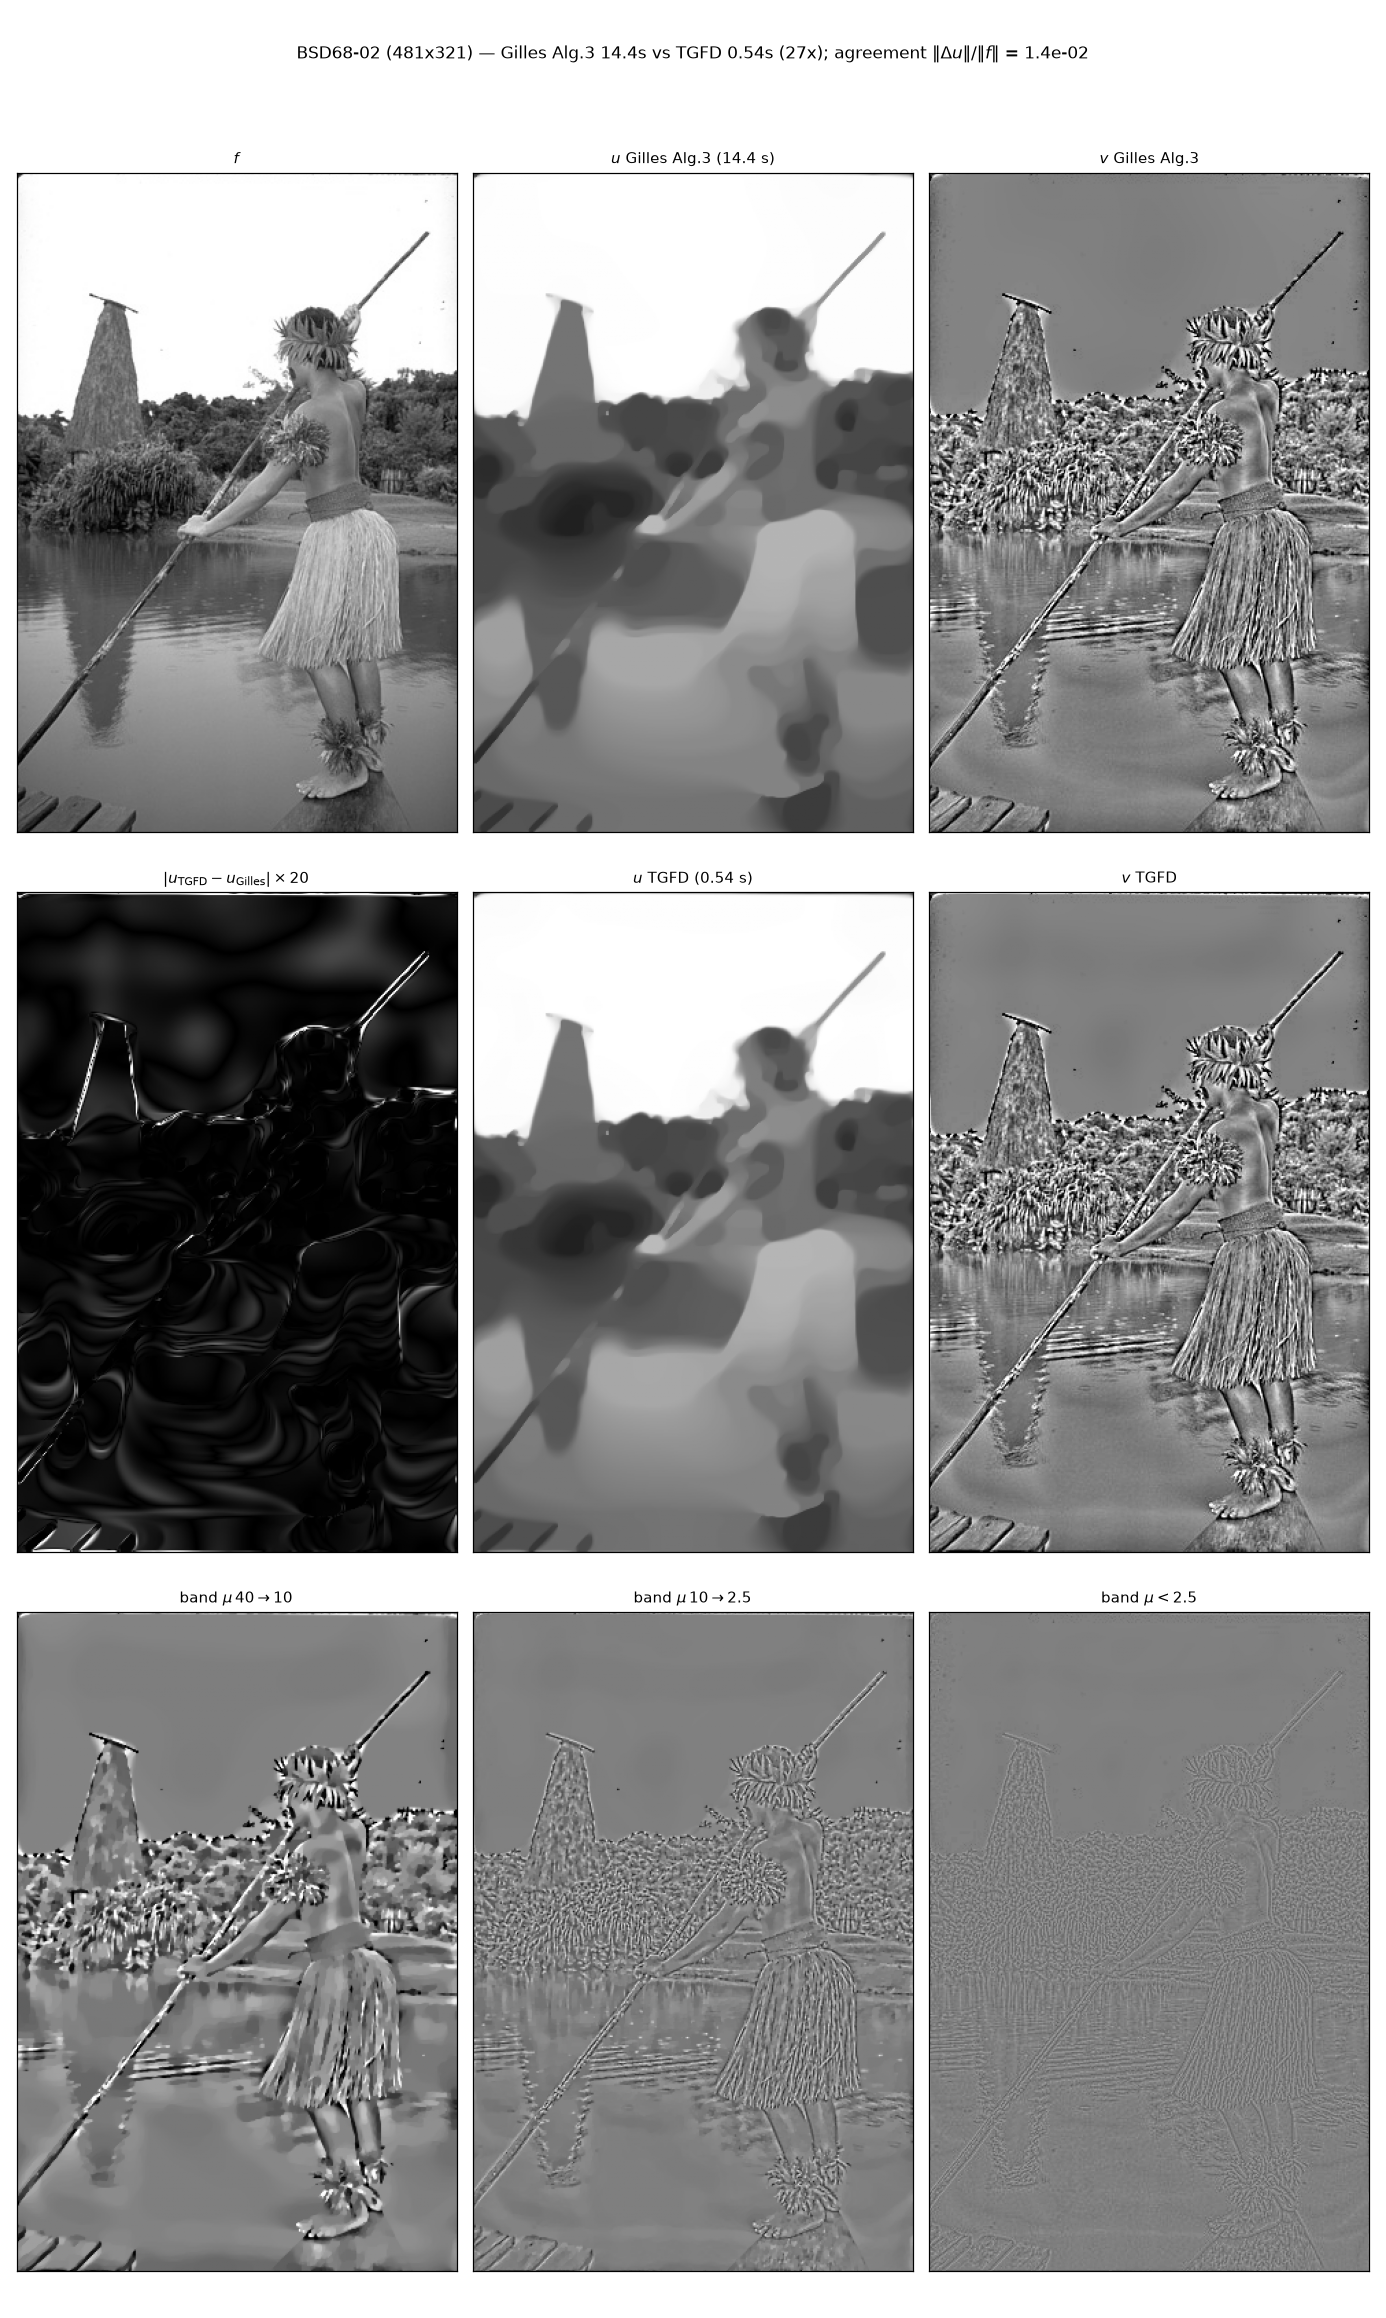
\includegraphics[width=\textwidth,height=0.9\textheight,keepaspectratio]{bsd68_002.png}
\captionof{figure}{BSD68-02, $481\times321$.}
\end{center}
\clearpage

\begin{center}
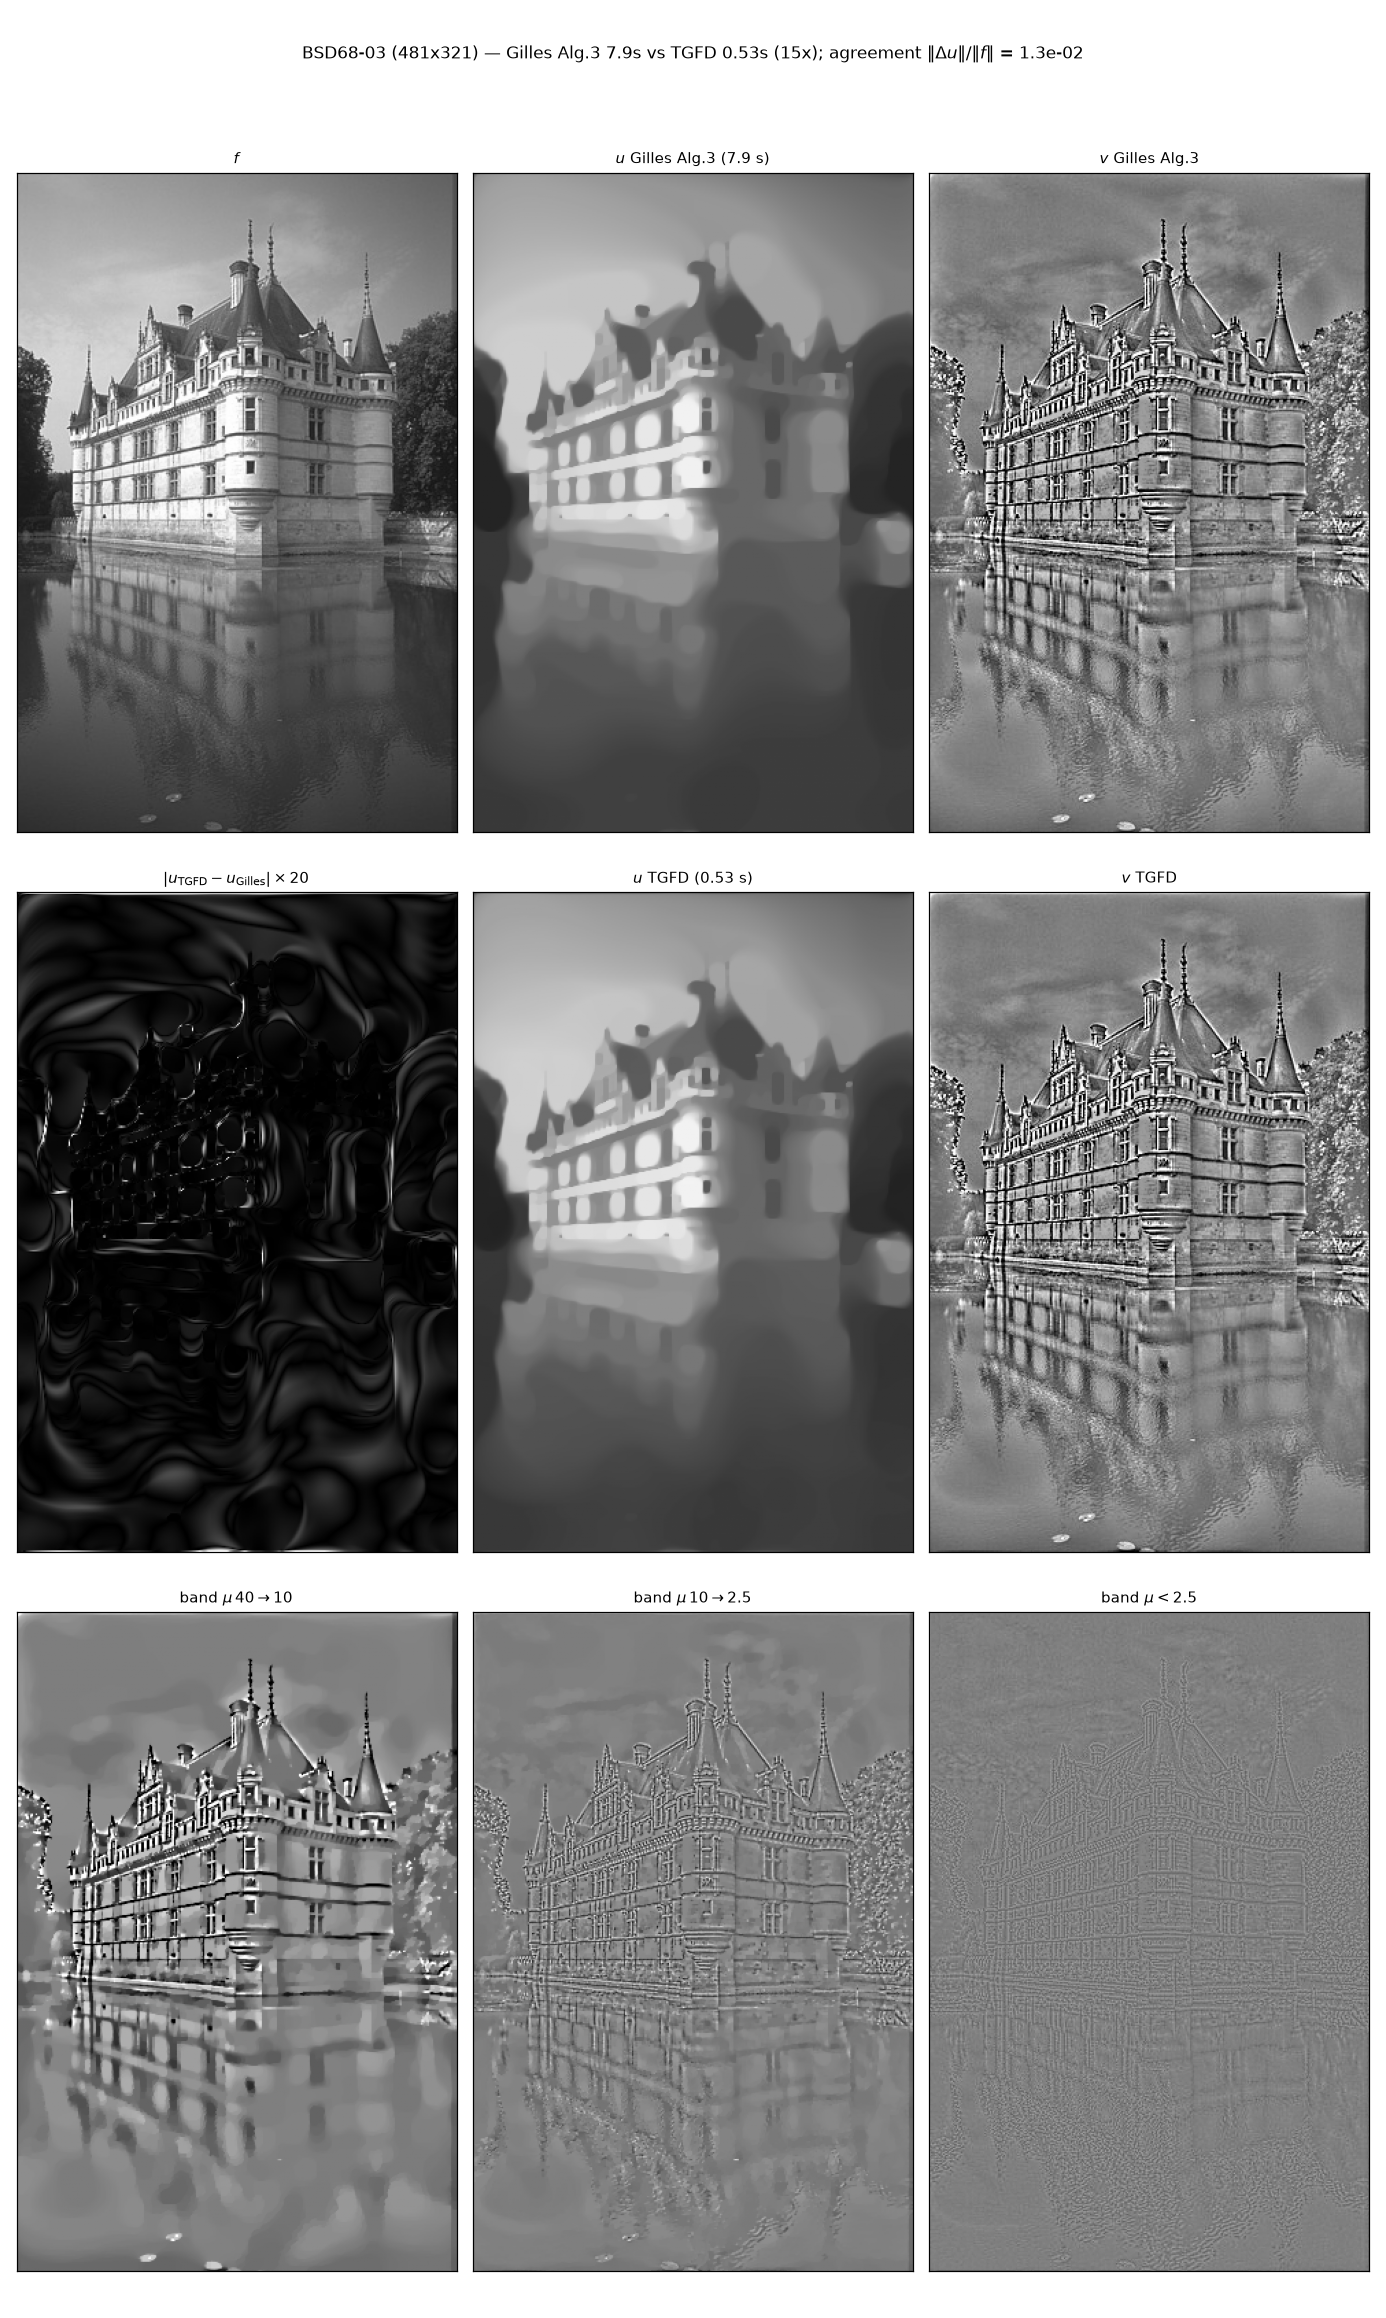
\includegraphics[width=\textwidth,height=0.9\textheight,keepaspectratio]{bsd68_003.png}
\captionof{figure}{BSD68-03, $481\times321$.}
\end{center}
\clearpage

\begin{center}
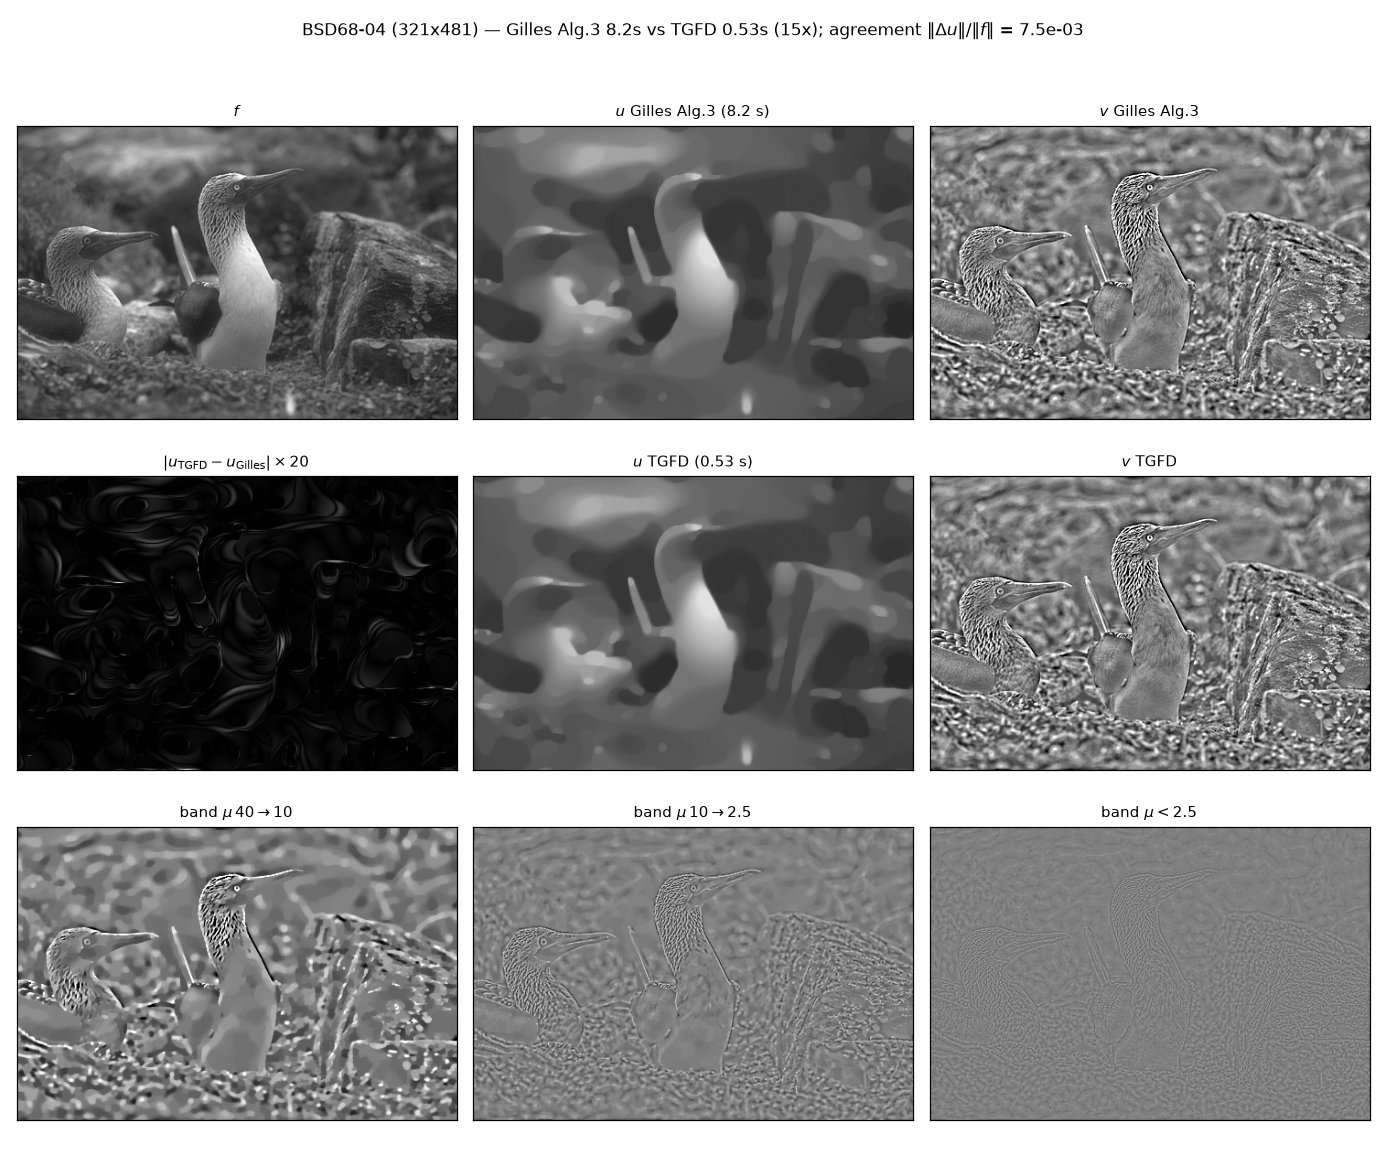
\includegraphics[width=\textwidth,height=0.9\textheight,keepaspectratio]{bsd68_004.png}
\captionof{figure}{BSD68-04, $321\times481$. Plumage in the mid band; rock texture
in the coarse and mid bands; the cartoon retains the animals' pose
structure.}
\end{center}
\clearpage

\begin{center}
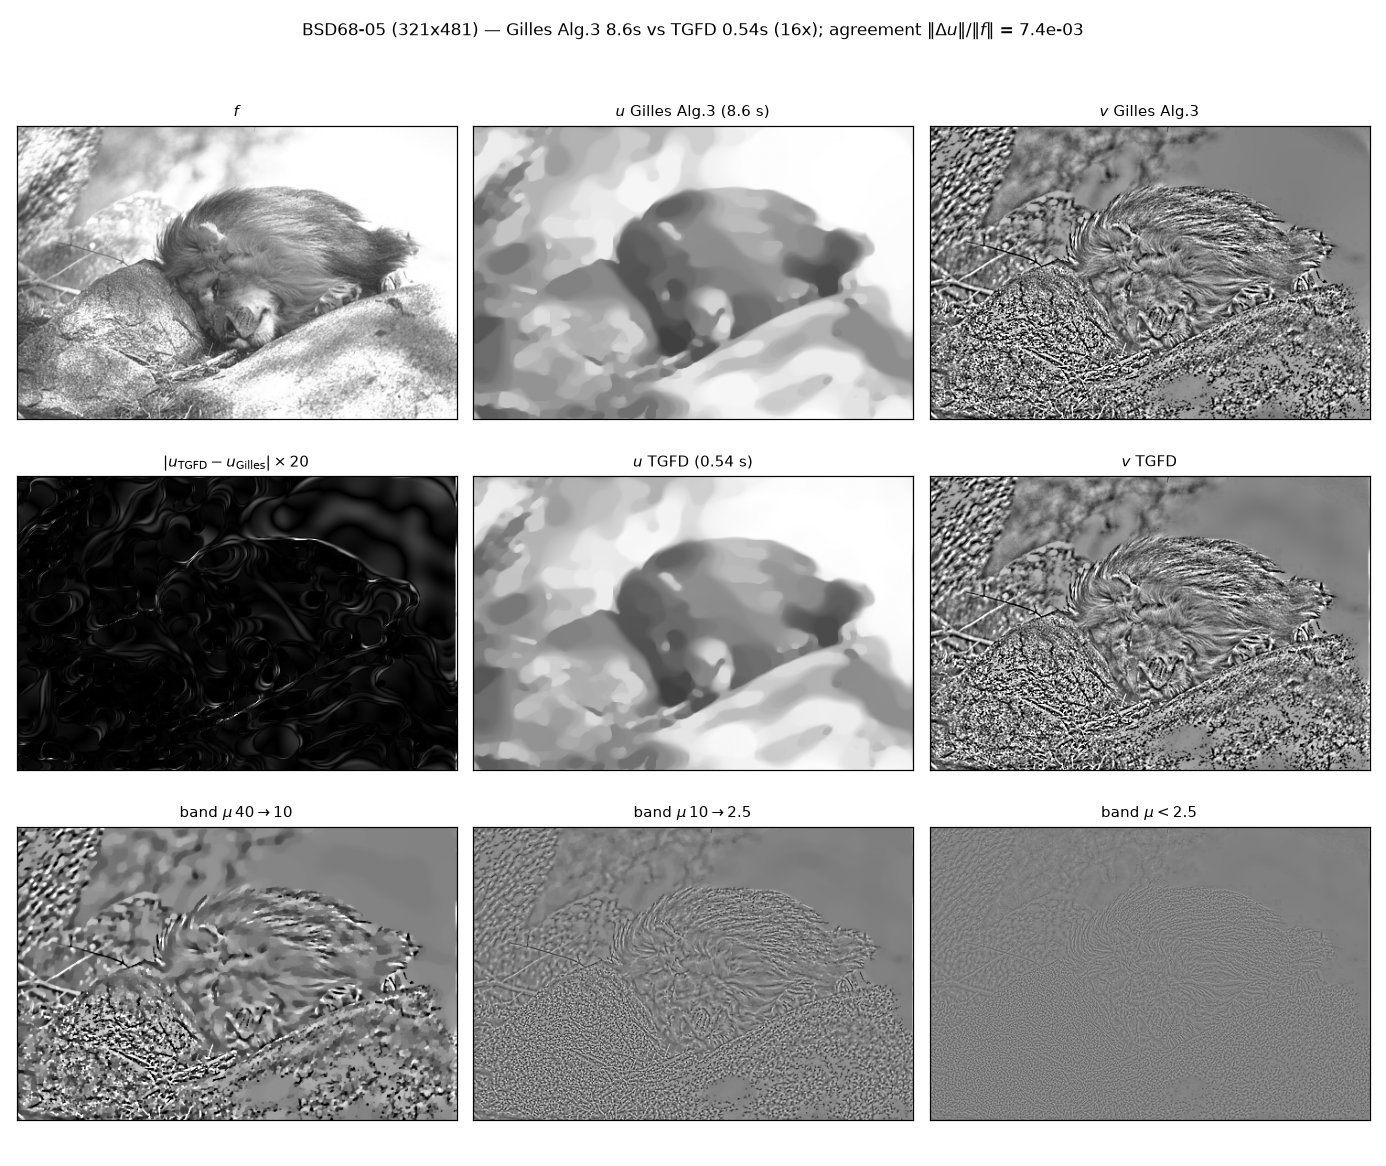
\includegraphics[width=\textwidth,height=0.9\textheight,keepaspectratio]{bsd68_005.png}
\captionof{figure}{BSD68-05, $321\times481$.}
\end{center}
\clearpage

\begin{center}
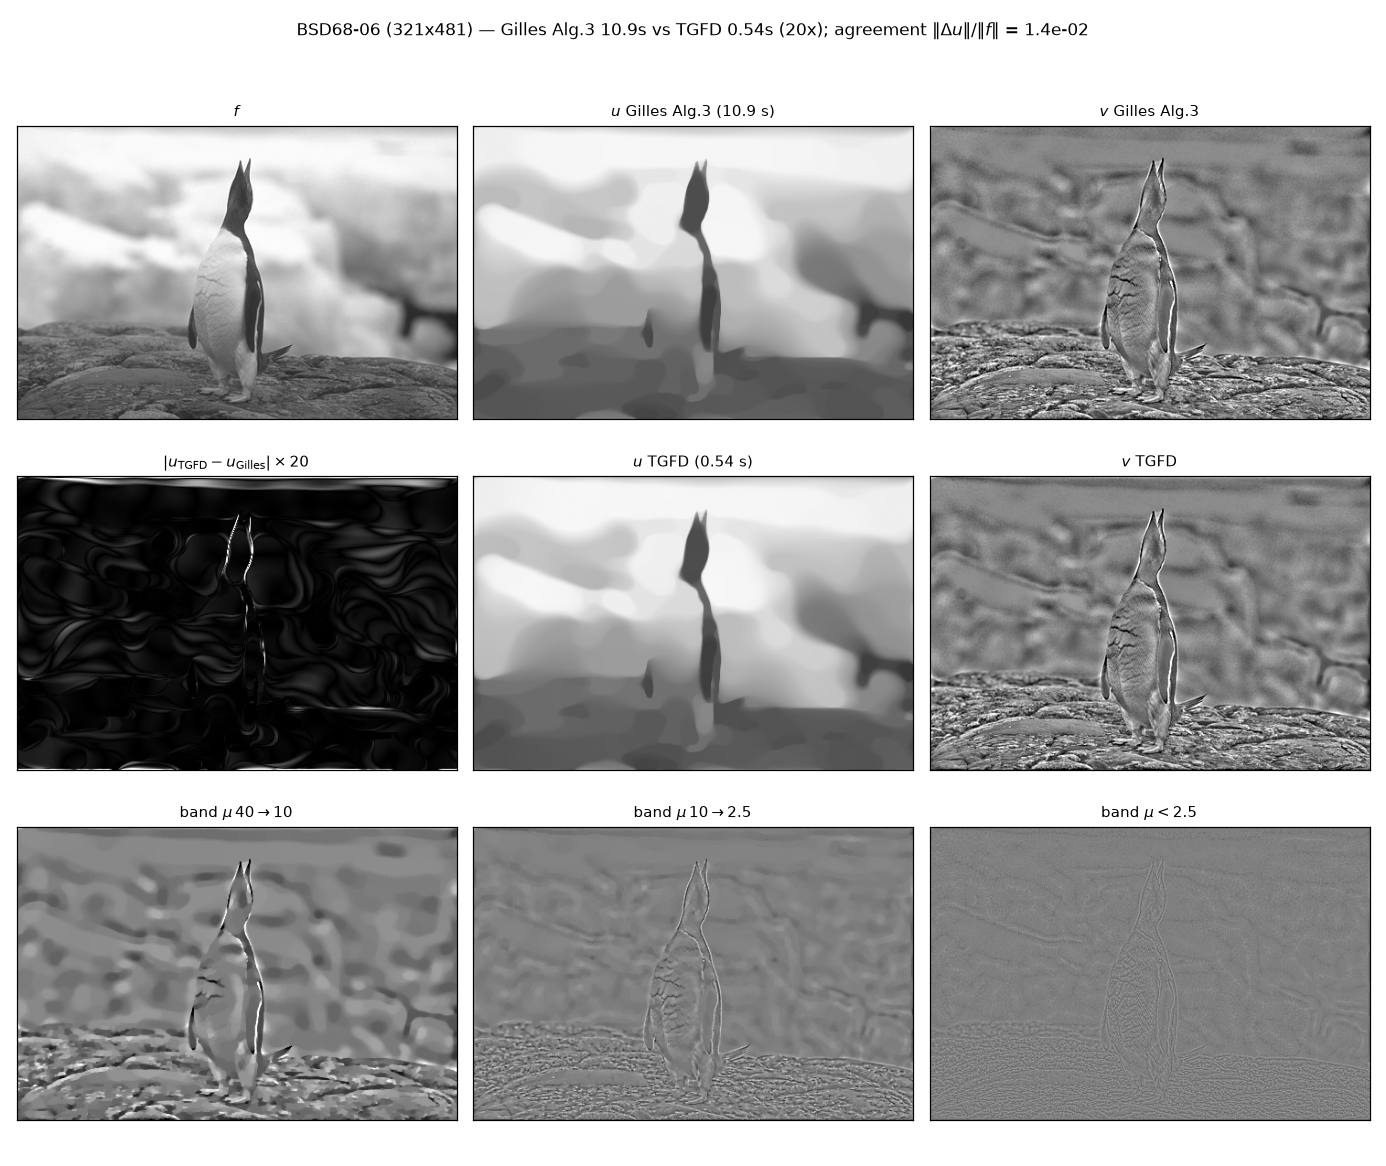
\includegraphics[width=\textwidth,height=0.9\textheight,keepaspectratio]{bsd68_006.png}
\captionof{figure}{BSD68-06, $321\times481$.}
\end{center}
\clearpage

\begin{center}
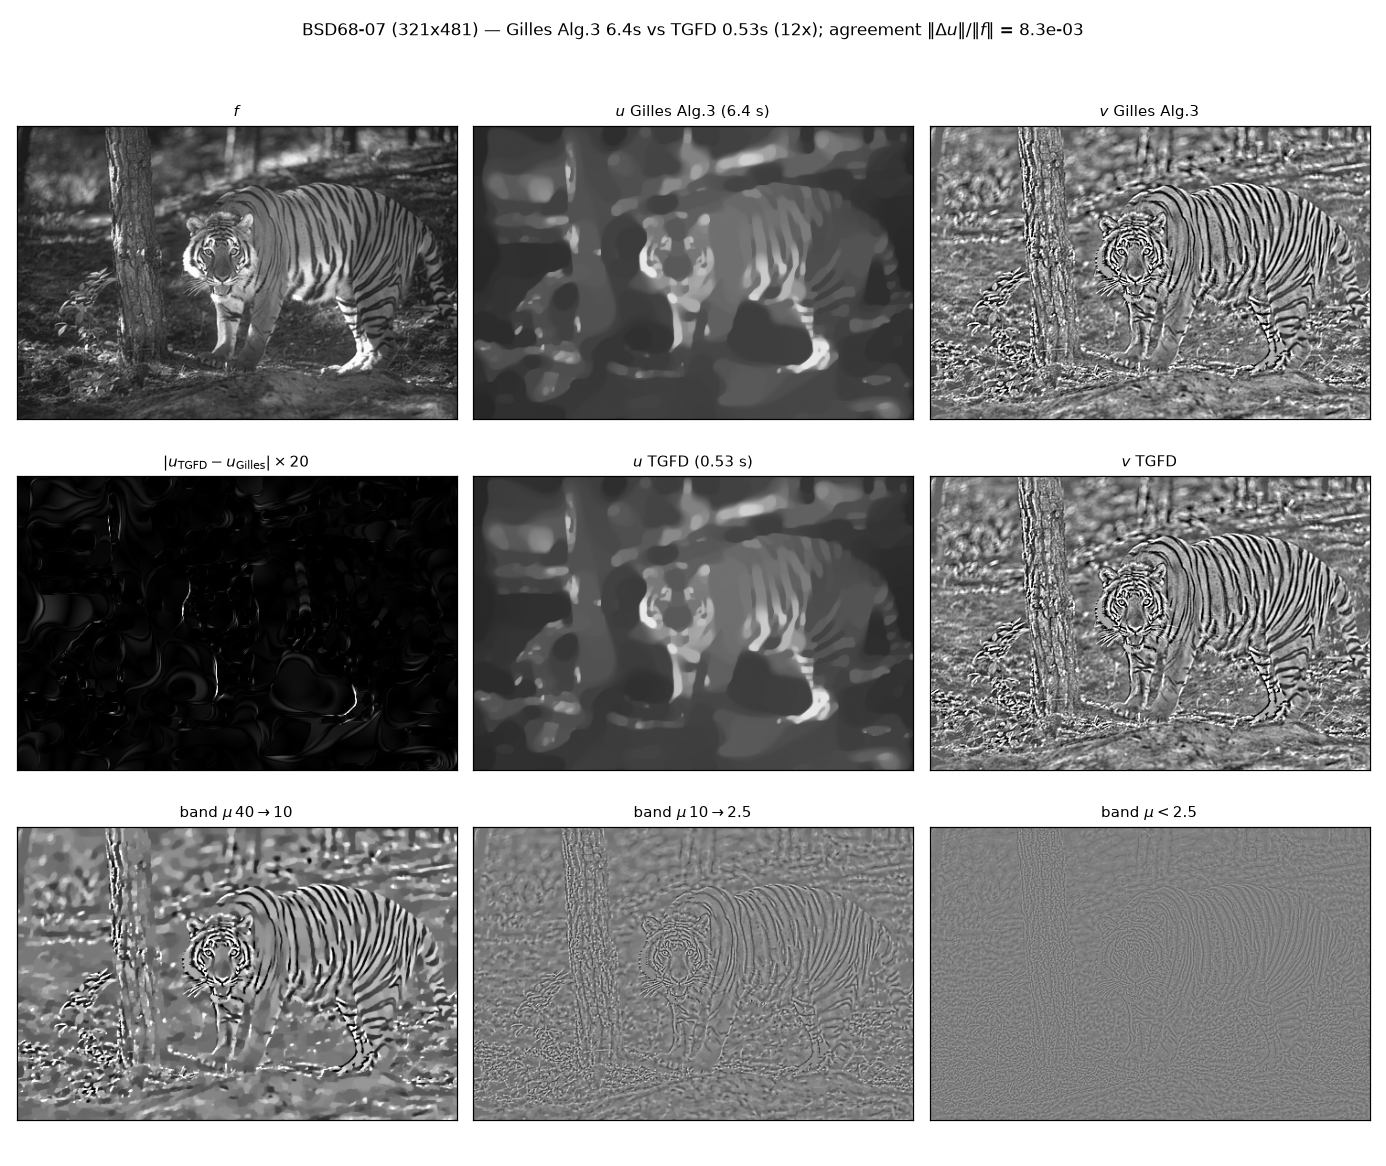
\includegraphics[width=\textwidth,height=0.9\textheight,keepaspectratio]{bsd68_007.png}
\captionof{figure}{BSD68-07, $321\times481$.}
\end{center}
\clearpage

\begin{center}
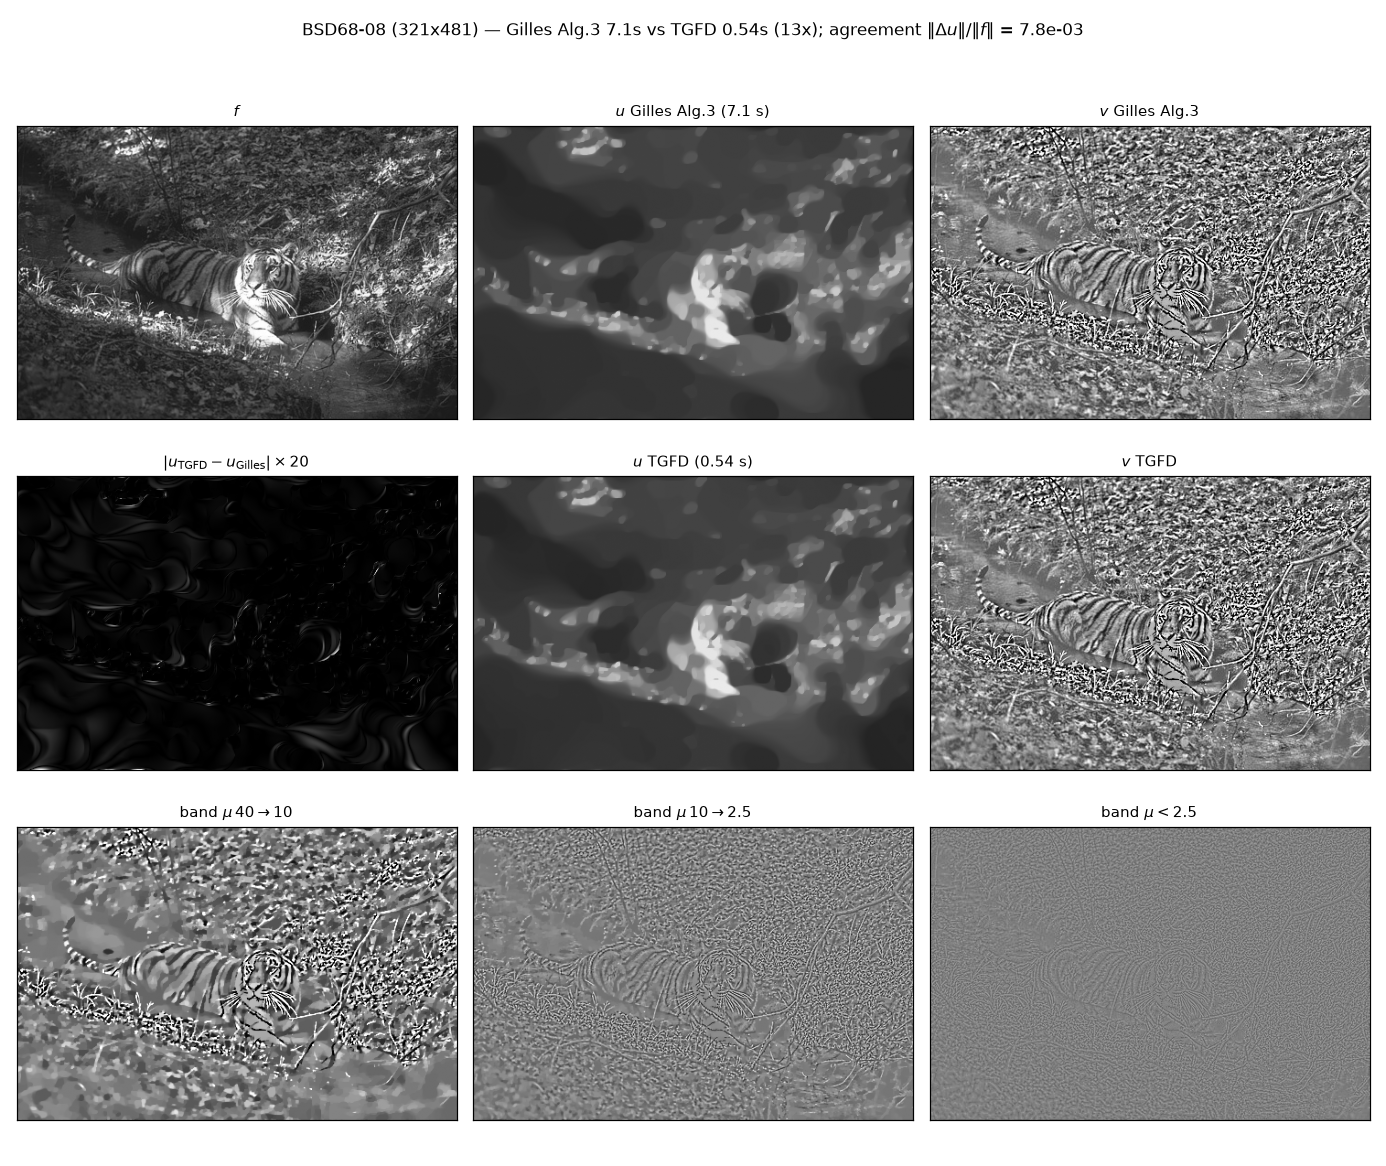
\includegraphics[width=\textwidth,height=0.9\textheight,keepaspectratio]{bsd68_008.png}
\captionof{figure}{BSD68-08, $321\times481$.}
\end{center}
\clearpage

\end{document}
